% Plain-language review document (explaneat plain-language review), v5.
\documentclass[a4paper,10pt]{article}
\usepackage[margin=1.8cm]{geometry}
\usepackage{amsmath}
\usepackage{amssymb}
\usepackage{booktabs}
\usepackage{tabularx}
\usepackage{graphicx}
\usepackage[table,usenames,dvipsnames]{xcolor}
\usepackage{tikz}
\usetikzlibrary{arrows.meta,fit,backgrounds,positioning,calc}
\usetikzlibrary{shapes.geometric}
\usepackage{longtable}
\usepackage{pdflscape}
\usepackage{float}
\usepackage[font=small,labelfont=bf]{caption}
\usepackage{array}
\usepackage[unicode=true,hidelinks]{hyperref}
\setcounter{tocdepth}{3}
\setcounter{secnumdepth}{3}
% Review markers, copied from dissertation.tex (7 Nov 2026) for standalone builds.
\newif\ifreviewmarks
\reviewmarkstrue
\newcommand{\reviewrule}{\noindent{\color{BrickRed}\rule{\linewidth}{0.8pt}}}
\newenvironment{drafted}[1][]{%
  \ifreviewmarks\par\addvspace{\medskipamount}\reviewrule\par\nopagebreak
  \noindent{\color{BrickRed}\sffamily\footnotesize\textbf{Thesis Draft}\quad #1\hfill review}\par\nopagebreak\smallskip\fi}{%
  \ifreviewmarks\par\smallskip\noindent{\color{BrickRed}\sffamily\footnotesize end of thesis draft}\par\nopagebreak\reviewrule\par\medskip\fi}
\newcommand{\figreview}[1]{\ifreviewmarks\par\smallskip{\color{NavyBlue}\sffamily\footnotesize\textbf{Figure note:} #1}\par\fi}
\begin{document}
\begin{center}{\Large\bfseries Plain-language explanation: heart-s1-c1\par}\vspace{2mm}{\small AI-assisted drafts for review. Nothing here has been verified by a person.\par}\end{center}
\noindent\textbf{How to read this.} Explanations are built up but read down: the summary first, then each part from the whole model down, in plain words, each sentence followed by the claims it rests on (C01, C02, \ldots; every cited claim was computed on the model and checked). Numbers are changes in predicted risk for a typical patient. The technical record (original hypotheses, formulas, evidence tables with the test check, ranges and n) is at the end. The text describes what the model does, not the world; whether it is plausible is for the reviewer to judge.
\par\medskip\noindent\textbf{What changed in v5e (figures).} v5e: every diagram is a numbered figure with a caption (list of figures after the contents) and the text refers to it; the whole-network figure has its own landscape page, scaled to the page, with a short caption and its description in the text; an input used by several parts is drawn under each of them (same input, repeated for readability, dotted outline); and an appendix figure shows the trained network before any explanation (no parts, no splits).
\par\medskip\noindent\textbf{What changed in v5c (tables and diagrams).} v5c: the evidence tables are landscape, compact and shaded by row, with the header repeated on every page (longtable and pdflscape, used in this review PDF only; the thesis preamble has neither). In the diagrams each input is drawn once, in a shared row along the bottom (the explanation's split copies of an input are listed in the technical detail instead), every cluster has one output rectangle with its plain name, the inputs that feed the output directly meet in a drawn 'sum', and a one-line legend explains the edges.
\par\medskip\noindent\textbf{What changed in v5b (diagrams).} v5b uses one grouping everywhere, the annotation hierarchy: the summary's diagram is the same picture as the whole model's section, and a part that is itself a weighted sum (blood pressure with cholesterol) is a part of its own, described as one that adds up, so the text counts three parts throughout; the lint checks every 'N parts' against the hierarchy. A full-structure diagram follows the summary: every node and connection, nested by part, with the inputs that feed the output directly in their own cluster and the unused input columns listed. Each section from the top down adds its own region of that diagram, with stubs for connections from or to other parts; each connection is drawn in exactly one section. The gate's text now says that it lowers the risk for the patients it acts on, and that more vessels and higher cholesterol take that lowering away; its vessel statements are one per group.
\par\medskip\noindent\textbf{What changed in v5 (read down).} v5 reads the explanation down. The summary (one line, a diagram, one paragraph per block) is as in v4, except that the paragraph on what adds up is split into protective items, risk-raising items and rare results, and an input that also feeds a part is quoted with its direct contribution only (the rest is in that part's paragraph). Then the document walks the annotation hierarchy from the whole model down: for each part a plain hypothesis (what it does for the prediction), plain evidence (what was checked and what it showed; for a part made of others, what they are and how they combine), a diagram one level down and where to read on. The original hypotheses, closed forms and evidence tables are in 'Technical detail' at the end. Statements about structure (what a part is made of, a copy of another part, a formula that reproduces it) are now claims of their own, checked on the graph and the data.
\par\medskip\noindent\textbf{v4.} v4 follows the structure of the explanation. The summary opens with one line and a diagram at the same grouping, then gives one paragraph per top-level block of the annotation hierarchy: one for everything that adds up independently (the inputs that feed the model score directly, and parts that are a weighted sum), and one for each part that combines its inputs in another way: what it combines, how, and for whom. 'Parts in detail' follows the hierarchy below that, with a diagram one level down for each part that contains others. The prose no longer says 'clearly', 'slightly', 'consistently' or 'on the training data only': the numbers carry it, and the test check, the ranges and n stay in the evidence tables. Only genuinely small groups are marked, with their n. The lint rejects the confidence words and checks the block structure.
\tableofcontents
\listoffigures
\clearpage
\begin{drafted}[plain-language layer: heart-s1-c1]
\section{heart-s1-c1}
\noindent{\small Genome \texttt{a2df22ce-983d-47b6-bbd6-3176d38ed5ff}, explanation \texttt{492866e6-a73b-4465-92a8-ecad82a2adcc}. Split: train primary (n=242), test as a check (n=61). Claims: 47, verified 47, not supported 0.\par}
\noindent{\small\textcolor{BrickRed}{AI-assisted draft for review (unverified)}\par}\smallskip
\noindent{\footnotesize Reference (typical) patient: the typical patient: the median training patient for every number and the most common training category for every category (not a real patient). age: 56 years; ca: 0 vessels; chol: 240 mg/dL (6.2 mmol/L); cp: no chest pain (asymptomatic); exang: no chest pain on exercise; fbs: fasting blood sugar of 120 mg/dL or less; oldpeak: 0.8 mm; restecg: a normal resting ECG; sex: male; slope: an upsloping ST segment; thal: a normal thallium scan; thalach: 152 beats per minute; trestbps: 130 mm Hg. Predicted risk of heart disease: 18\%.\par}
\subsection{Summary}
\noindent For a typical patient (a 56-year-old man with no chest pain symptoms and median test results) the model predicts a risk of heart disease of about 18\%; it adds up most of its inputs independently, and five parts add to that sum: two add more for each extra vessel coloured, one lowers the risk for typical angina, one lowers it for non-anginal chest pain, one acts only on the 42 of 242 training patients with a normal resting ECG and marked ST depression, and one lowers it for a higher maximum heart rate, with nothing until about 145 beats per minute, then steadily.\,{\scriptsize\textcolor{NavyBlue}{[C29, C30, C40, C31, C43, C38, C46]}} Figure~\ref{fig:hearts1c1:summary} shows the model at this level: one box per paragraph below.
\par\medskip\noindent\fbox{\begin{minipage}{0.96\linewidth}\small\textbf{How to read the diagrams.} Edge colour is the sign of that one connection: blue positive, red negative; thicker is a larger weight. The outline and arrow on an input (and on a part's output box) is its overall effect on the final prediction, read from the verified claims: orange and up arrow raises it, teal and down arrow lowers it, grey and double arrow depends (it goes both ways, or differs between levels). A negative connection into a part that itself raises the prediction means that input lowers the prediction; through a hinge the overall effect can only be read from the claims, not from the edges. Up arrow means towards heart disease; down arrow, away from it. A double outline marks an input (or a part's output) that acts at a fixed rate everywhere: it adds the same amount to the score per unit, so it is explained by its rate alone (see 'Linear factors'); a dashed double outline, at a fixed rate on the observed data. The normal outline is an input whose effect switches on and off somewhere. For example, normal ECG has a positive connection into 'ST depression with a normal ECG', a part that raises the predicted risk of heart disease, so normal ECG raises it.\end{minipage}}\par\medskip
\begin{figure}[H]\centering
\resizebox{!}{\ifdim\height>0.5\textheight 0.5\textheight\else\height\fi}{%
\resizebox{\ifdim\width>\linewidth\linewidth\else\width\fi}{!}{%
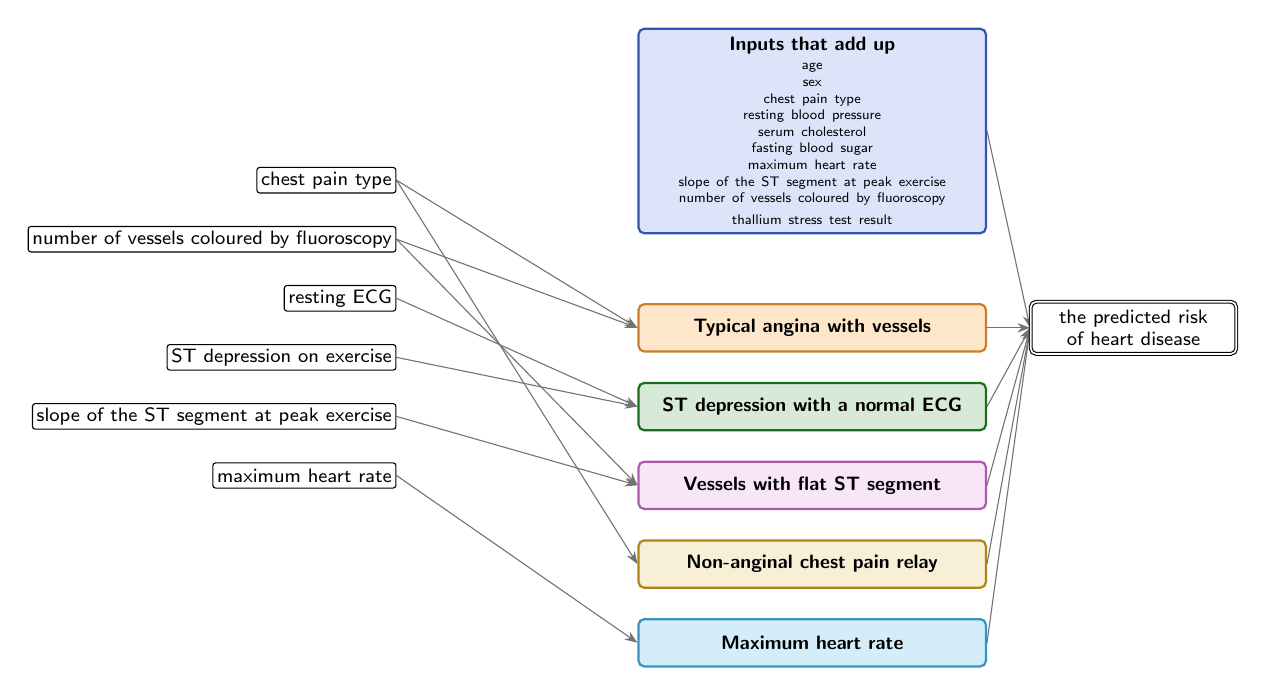
\begin{tikzpicture}[
  font=\sffamily\scriptsize, >={Stealth[length=1.6mm]},
  inp/.style={draw, rounded corners=1pt, fill=white, inner sep=1.5pt, minimum height=3.2mm, anchor=east},
  abox/.style={draw, thick, rounded corners=2pt, align=center, inner sep=3pt, minimum height=6mm, text width=42mm},
  outp/.style={draw, double, rounded corners=2pt, fill=white, align=center, inner sep=3pt, text width=24mm},
  agg/.style={draw=black!55},
]
\node[inp] (i0) at (0,1.875) {chest pain type};
\node[inp] (i1) at (0,1.125) {number of vessels coloured by fluoroscopy};
\node[inp] (i2) at (0,0.375) {resting ECG};
\node[inp] (i3) at (0,-0.375) {ST depression on exercise};
\node[inp] (i4) at (0,-1.125) {slope of the ST segment at peak exercise};
\node[inp] (i5) at (0,-1.875) {maximum heart rate};
\node[abox, fill=RoyalBlue!18, draw=RoyalBlue!80!black] (b0) at (5.28,2.5) {\textbf{Inputs that add up}\\[1pt]{\tiny age\\ sex\\ chest pain type\\ resting blood pressure\\ serum cholesterol\\ fasting blood sugar\\ maximum heart rate\\ slope of the ST segment at peak exercise\\ number of vessels coloured by fluoroscopy\\ thallium stress test result}};
\node[abox, fill=BurntOrange!18, draw=BurntOrange!80!black] (b1) at (5.28,-0.0) {\textbf{Typical angina with vessels}};
\node[abox, fill=ForestGreen!18, draw=ForestGreen!80!black] (b2) at (5.28,-1.0) {\textbf{ST depression with a normal ECG}};
\node[abox, fill=Orchid!18, draw=Orchid!80!black] (b3) at (5.28,-2.0) {\textbf{Vessels with flat ST segment}};
\node[abox, fill=Goldenrod!18, draw=Goldenrod!80!black] (b4) at (5.28,-3.0) {\textbf{Non-anginal chest pain relay}};
\node[abox, fill=Cerulean!18, draw=Cerulean!80!black] (b5) at (5.28,-4.0) {\textbf{Maximum heart rate}};
\node[outp] (out) at (9.36,0) {the predicted risk of heart disease};
\begin{scope}[on background layer]
\draw[->, agg] (b0.east) -- (out.west);
\draw[->, agg, thin] (i0.east) -- (b1.west);
\draw[->, agg, thin] (i1.east) -- (b1.west);
\draw[->, agg] (b1.east) -- (out.west);
\draw[->, agg, thin] (i2.east) -- (b2.west);
\draw[->, agg, thin] (i3.east) -- (b2.west);
\draw[->, agg] (b2.east) -- (out.west);
\draw[->, agg, thin] (i4.east) -- (b3.west);
\draw[->, agg, thin] (i1.east) -- (b3.west);
\draw[->, agg] (b3.east) -- (out.west);
\draw[->, agg, thin] (i0.east) -- (b4.west);
\draw[->, agg] (b4.east) -- (out.west);
\draw[->, agg, thin] (i5.east) -- (b5.west);
\draw[->, agg] (b5.east) -- (out.west);
\end{scope}
\end{tikzpicture}}}%
\caption{The model at the level of the summary: one box per part.}
\label{fig:hearts1c1:summary}
\end{figure}
\paragraph{Inputs that add up.} \par\noindent\textit{Lowering the risk.}  These add up independently, and these lower the risk: being a woman takes a typical patient's predicted risk from about 18\% to below 1\% and fasting blood sugar above 120 mg/dL to about 8\%; through this sum alone, compared with no chest pain symptoms, typical angina or non-anginal chest pain lowers it to about 2\% and atypical angina to about 5\% (chest pain type also acts through the parts below).\,{\scriptsize\textcolor{NavyBlue}{[C10, C19, C12, C17]}} \par\noindent\textit{Raising the risk.}  A reversible defect (or the undefined code 4) on the thallium scan raises it to about 55\%; higher cholesterol (from about 8\% at 193 mg/dL to about 45\% at 308 mg/dL), higher resting blood pressure (from about 9\% at 110 mm Hg to about 35\% at 155 mm Hg) and older age (from about 10\% at 42 years to about 25\% at 66 years) raise it steadily.\,{\scriptsize\textcolor{NavyBlue}{[C05, C07, C08, C13]}} Through this sum alone, each extra vessel coloured by fluoroscopy adds about the same (from about 18\% at 0 to about 80\% at 2 vessels) and a flat ST segment raises it to about 87\%, while the maximum heart rate barely changes it; all three also act through the parts below.\,{\scriptsize\textcolor{NavyBlue}{[C04, C03, C21]}} \par\noindent\textit{Rare results.}  Rarer results also count (the model has little data on this, n = 15 and 17): a fixed defect on the thallium scan lowers the risk to about 3\%, and through this sum alone a downsloping ST segment raises it to about 32\%; the model ignores exercise-induced angina.\,{\scriptsize\textcolor{NavyBlue}{[C14, C15, C28]}}
\paragraph{Typical angina with vessels.} This part combines chest pain type with the number of vessels coloured: through it, typical angina lowers a typical patient's predicted risk from about 18\% to about 2\%, and each extra vessel adds about the same, from about 18\% at 0 to about 61\% at 2 vessels.\,{\scriptsize\textcolor{NavyBlue}{[C31, C30]}} Across the whole model, more vessels raise the predicted risk, and even more so with typical angina, each extra vessel adding about the same: going from 0 to 2 vessels moves a typical patient from below 1\% to about 55\% with typical angina, and from about 18\% to about 99\% with any other chest pain type.\,{\scriptsize\textcolor{NavyBlue}{[C32]}} Across the whole model, typical angina takes a typical patient's predicted risk to below 1\%.\,{\scriptsize\textcolor{NavyBlue}{[C09]}}
\paragraph{ST depression with a normal ECG.} This part combines the resting ECG with ST depression on exercise and acts on 42 of 242 training patients, nearly all with a normal resting ECG, 26 of whom had heart disease; for the typical patient it acts on, the predicted risk is about 98\% without it and about 99\% with it.\,{\scriptsize\textcolor{NavyBlue}{[C38]}} Through it, more ST depression raises the predicted risk only once it rises above about 1.0 mm, for patients with a normal resting ECG, in an uneven way: for a typical such patient from about 13\% at 0 mm to about 63\% at 3.5 mm.\,{\scriptsize\textcolor{NavyBlue}{[C37]}} More ST depression therefore raises the predicted risk, but only if the resting ECG is normal: going from 0 to 2.8 mm moves a typical patient from about 18\% to about 55\% with a normal resting ECG, in an uneven way, and leaves it at about 18\% otherwise.\,{\scriptsize\textcolor{NavyBlue}{[C36]}}
\paragraph{Vessels with flat ST segment.} This part combines the number of vessels coloured with a flat ST segment: through it, each extra vessel adds about the same, from about 18\% at 0 to about 36\% at 2 vessels for a typical patient, and a flat ST segment raises the risk from about 18\% to about 23\%.\,{\scriptsize\textcolor{NavyBlue}{[C40, C41]}} Across the whole model, each extra vessel takes a typical patient from about 18\% at 0 to about 99\% at 2 vessels, about the same for each, flattening out near the top because the predicted risk cannot go much higher, and a flat ST segment takes it to about 91\%.\,{\scriptsize\textcolor{NavyBlue}{[C01, C02]}}
\paragraph{Non-anginal chest pain relay.} This part reads only non-anginal chest pain: through it, non-anginal chest pain lowers a typical patient's predicted risk from about 18\% to about 8\%.\,{\scriptsize\textcolor{NavyBlue}{[C43]}} Across the whole model, non-anginal chest pain takes it to about 1\%.\,{\scriptsize\textcolor{NavyBlue}{[C11]}}
\paragraph{Maximum heart rate.} This part reads only the maximum heart rate: a higher maximum heart rate lowers the predicted risk with nothing until about 145 beats per minute, then steadily, for a typical patient from about 19\% at 118 to about 14\% at 175 beats per minute.\,{\scriptsize\textcolor{NavyBlue}{[C45, C46]}} Across the whole model the same holds, from about 19\% at 118 to about 14\% at 175 beats per minute.\,{\scriptsize\textcolor{NavyBlue}{[C20]}}
\paragraph{The whole network.} Figure~\ref{fig:hearts1c1:overview} (next page, landscape) draws every unit and connection of the explained model, nested by part: shaded clusters are the parts of the model and darker boxes the parts inside them; circles are hidden units (h1, h2, \ldots); each cluster's rectangle is its output, and a dashed `sum' stands for an addition the next unit does (drawn, not a unit of the model); the hexagon is the model's output. An input used by several parts is drawn under each of them (same label, dotted outline, the first copy marked with the number of copies): it is the same input, repeated for readability. Not used by the model (input columns with no connection): male, sugar 120 or less, ST-T abnormal ECG, LVH on ECG, no exercise pain, exercise pain, upsloping ST, thallium code 4, reversible defect.
\begin{landscape}
\begin{figure}[p]\centering
\resizebox{\linewidth}{!}{%
\definecolor{netup}{HTML}{D95F02}\definecolor{netdown}{HTML}{1B9E77}\definecolor{netmixed}{HTML}{7F7F7F}%
\begin{tikzpicture}[
  font=\sffamily\scriptsize, >={Stealth[length=1.4mm]},
  inp/.style={draw, circle, fill=white, minimum size=3.2mm, inner sep=0pt},
  hid/.style={draw, circle, fill=white, minimum size=5.2mm, inner sep=0.5pt, font=\sffamily\tiny},
  exitbox/.style={draw, thick, rectangle, fill=white, align=center, text width=17mm, minimum height=5mm, inner sep=1.5pt, font=\sffamily\tiny},
  sumbox/.style={draw, thick, dashed, rectangle, fill=white, align=center, text width=17mm, minimum height=5mm, inner sep=1.5pt, font=\sffamily\tiny},
  outp/.style={draw, thick, regular polygon, regular polygon sides=6, fill=white, minimum size=10mm, inner sep=0pt, font=\sffamily\tiny, align=center},
  stub/.style={draw, dashed, rounded corners=2pt, fill=white, align=center, inner sep=2pt, font=\sffamily\tiny, text width=15mm},
  inlab/.style={font=\sffamily\tiny, align=center, text width=15mm, inner sep=1pt, fill=white, fill opacity=0.8, text opacity=1},
  wpos/.style={draw=NavyBlue}, wneg/.style={draw=BrickRed}, wagg/.style={draw=black!45, line width=1.2pt},
  wmix/.style={draw=Plum},
]
\node[outp] (n0) at (22.45,6.15) {heart disease};
\node[exitbox] (n1173) at (37.86,1.9) {Non-anginal chest pain relay $\downarrow$};
\node[exitbox] (n1801) at (23.28,1.9) {ST depression with a normal ECG $\uparrow$};
\node[hid] (n2009) at (44.0,1.9) {h4};
\node[hid] (n2245) at (15.94,1.9) {h5};
\node[hid] (n2650) at (44.0,3.25) {h6};
\node[hid] (n3210) at (15.94,3.25) {h7};
\node[exitbox] (n664) at (30.72,1.9) {Vessels with flat ST segment $\uparrow$};
\node[sumbox] (ncsumxxannx32) at (44.0,4.6) {sum: Maximum heart rate $\downarrow$};
\node[sumbox] (ncsumxxannx33) at (15.94,4.6) {sum: Typical angina with vessels $\updownarrow$};
\node[sumbox] (nxxsumxx) at (5.85,1.9) {sum: Inputs that add up};
\node[inp, draw=netup, very thick] (ninxxagexxadditive) at (0.9,0.0) {};
\path (ninxxagexxadditive.south) node[inlab, anchor=north] (labninxxagexxadditive) {age $\uparrow$};
\node[inp, draw=netdown, very thick] (ninxxsexx0xxadditive) at (4.5,0.0) {};
\path (ninxxsexx0xxadditive.south) node[inlab, anchor=north] (labninxxsexx0xxadditive) {female $\downarrow$};
\node[inp, draw=netdown, very thick] (ninxxcpx2xxadditive) at (0.9,-2.1) {};
\path (ninxxcpx2xxadditive.south) node[inlab, anchor=north] (labninxxcpx2xxadditive) {atypical angina $\downarrow$};
\node[inp, draw=netup, very thick] (ninxxcpx4xxadditive) at (8.1,0.0) {};
\path (ninxxcpx4xxadditive.south) node[inlab, anchor=north] (labninxxcpx4xxadditive) {no chest pain $\uparrow$};
\node[inp, draw=netup, very thick] (ninxxtrestbpsxxadditive) at (1.8,-1.05) {};
\path (ninxxtrestbpsxxadditive.south) node[inlab, anchor=north] (labninxxtrestbpsxxadditive) {blood pressure $\uparrow$};
\node[inp, draw=netup, very thick] (ninxxcholxxadditive) at (2.7,0.0) {};
\path (ninxxcholxxadditive.south) node[inlab, anchor=north] (labninxxcholxxadditive) {cholesterol $\uparrow$};
\node[inp, draw=netdown, very thick] (ninxxfbsx1xxadditive) at (9.9,0.0) {};
\path (ninxxfbsx1xxadditive.south) node[inlab, anchor=north] (labninxxfbsx1xxadditive) {sugar above 120 $\downarrow$};
\node[inp, draw=netup, very thick] (ninxxslopex3xxadditive) at (3.6,-1.05) {};
\path (ninxxslopex3xxadditive.south) node[inlab, anchor=north] (labninxxslopex3xxadditive) {downsloping ST $\uparrow$};
\node[inp, draw=netmixed, very thick] (ninxxthalx3xxadditive) at (9.0,-1.05) {};
\path (ninxxthalx3xxadditive.south) node[inlab, anchor=north] (labninxxthalx3xxadditive) {normal thallium $\updownarrow$};
\node[inp, draw=netdown, very thick] (ninxxthalx6xxadditive) at (5.4,-1.05) {};
\path (ninxxthalx6xxadditive.south) node[inlab, anchor=north] (labninxxthalx6xxadditive) {fixed defect $\downarrow$};
\node[inp, draw=netdown, very thick] (ninxxcpx1xxannx33) at (15.04,0.0) {};
\path (ninxxcpx1xxannx33.south) node[inlab, anchor=north] (labninxxcpx1xxannx33) {typical angina $\downarrow$};
\node[inp, draw=netdown, very thick] (ninxxcpx3xxannx30) at (37.86,0.0) {};
\path (ninxxcpx3xxannx30.south) node[inlab, anchor=north] (labninxxcpx3xxannx30) {non-anginal pain $\downarrow$};
\node[inp, draw=netup, very thick] (ninxxrestecgx0xxannx31) at (24.18,0.0) {};
\path (ninxxrestecgx0xxannx31.south) node[inlab, anchor=north] (labninxxrestecgx0xxannx31) {normal ECG $\uparrow$};
\node[inp, draw=netup, very thick] (ninxxoldpeakxxannx31) at (22.38,0.0) {};
\path (ninxxoldpeakxxannx31.south) node[inlab, anchor=north] (labninxxoldpeakxxannx31) {ST depression $\uparrow$};
\node[inp, densely dotted, thick, draw=netup, very thick] (ninxxcaxxadditive) at (10.8,-1.05) {};
\path (ninxxcaxxadditive.south) node[inlab, anchor=north] (labninxxcaxxadditive) {vessels ($\times$3) $\uparrow$};
\node[inp, densely dotted, thick, draw=netup, very thick] (ninxxcaxxannx29) at (31.62,0.0) {};
\path (ninxxcaxxannx29.south) node[inlab, anchor=north] (labninxxcaxxannx29) {vessels $\uparrow$};
\node[inp, densely dotted, thick, draw=netup, very thick] (ninxxcaxxannx33) at (16.84,0.0) {};
\path (ninxxcaxxannx33.south) node[inlab, anchor=north] (labninxxcaxxannx33) {vessels $\uparrow$};
\node[inp, densely dotted, thick, draw=netup, very thick] (ninxxslopex2xxadditive) at (6.3,0.0) {};
\path (ninxxslopex2xxadditive.south) node[inlab, anchor=north] (labninxxslopex2xxadditive) {flat ST ($\times$2) $\uparrow$};
\node[inp, densely dotted, thick, draw=netup, very thick] (ninxxslopex2xxannx29) at (29.82,0.0) {};
\path (ninxxslopex2xxannx29.south) node[inlab, anchor=north] (labninxxslopex2xxannx29) {flat ST $\uparrow$};
\node[inp, densely dotted, thick, draw=netup, very thick] (ninxxthalachxxadditive) at (7.2,-1.05) {};
\path (ninxxthalachxxadditive.south) node[inlab, anchor=north] (labninxxthalachxxadditive) {max heart rate ($\times$2) $\uparrow$};
\node[inp, densely dotted, thick, draw=netdown, very thick] (ninxxthalachxxannx32) at (44.0,0.0) {};
\path (ninxxthalachxxannx32.south) node[inlab, anchor=north] (labninxxthalachxxannx32) {max heart rate $\downarrow$};
\begin{scope}[on background layer]
\node[fit=(nxxsumxx) , inner sep=8pt, rounded corners=5pt, fill=RoyalBlue!10, draw=RoyalBlue!45] (clu0) {};
\node[fit=(n2245) (n3210) (ncsumxxannx33) , inner sep=8pt, rounded corners=5pt, fill=BurntOrange!10, draw=BurntOrange!45] (clu1) {};
\node[fit=(n1801) , inner sep=8pt, rounded corners=5pt, fill=ForestGreen!10, draw=ForestGreen!45] (clu2) {};
\node[fit=(n664) , inner sep=8pt, rounded corners=5pt, fill=Orchid!10, draw=Orchid!45] (clu3) {};
\node[fit=(n1173) , inner sep=8pt, rounded corners=5pt, fill=Goldenrod!10, draw=Goldenrod!45] (clu4) {};
\node[fit=(n2009) (n2650) (ncsumxxannx32) , inner sep=8pt, rounded corners=5pt, fill=Cerulean!10, draw=Cerulean!45] (clu5) {};
\draw[->, wpos, line width=0.39pt] (ninxxagexxadditive) -- (nxxsumxx);
\draw[->, wneg, line width=0.90pt] (ninxxsexx0xxadditive) -- (nxxsumxx);
\draw[->, wpos, line width=0.41pt] (ninxxcpx2xxadditive) -- (nxxsumxx);
\draw[->, wpos, line width=0.69pt] (ninxxcpx4xxadditive) -- (nxxsumxx);
\draw[->, wpos, line width=0.48pt] (ninxxtrestbpsxxadditive) -- (nxxsumxx);
\draw[->, wpos, line width=0.58pt] (ninxxcholxxadditive) -- (nxxsumxx);
\draw[->, wneg, line width=0.36pt] (ninxxfbsx1xxadditive) -- (nxxsumxx);
\draw[->, wpos, line width=0.32pt] (ninxxslopex3xxadditive) -- (nxxsumxx);
\draw[->, wneg, line width=0.55pt] (ninxxthalx3xxadditive) -- (nxxsumxx);
\draw[->, wneg, line width=0.55pt] (ninxxthalx6xxadditive) -- (nxxsumxx);
\draw[->, wpos, line width=0.57pt] (n664) -- (n0);
\draw[->, wneg, line width=0.68pt] (n1173) -- (n0);
\draw[->, wpos, line width=0.74pt] (n1801) -- (n0);
\draw[->, wneg, line width=0.30pt] (n2009) -- (ncsumxxannx32);
\draw[->, wpos, line width=0.78pt] (n2245) -- (ncsumxxannx33);
\draw[->, wneg, line width=0.31pt] (n2650) -- (ncsumxxannx32);
\draw[->, wneg, line width=0.54pt] (n3210) -- (ncsumxxannx33);
\draw[->, wpos, line width=0.57pt] (ninxxcpx1xxannx33) -- (n3210);
\draw[->, wpos, line width=0.37pt] (ninxxcpx3xxannx30) -- (n1173);
\draw[->, wpos, line width=0.79pt] (ninxxrestecgx0xxannx31) -- (n1801);
\draw[->, wpos, line width=0.54pt] (ninxxoldpeakxxannx31) -- (n1801);
\draw[->, wpos, line width=0.59pt] (n2009) -- (n2650);
\draw[->, wneg, line width=0.48pt] (n2245) -- (n3210);
\draw[->, wpos, line width=0.70pt] (ninxxcaxxadditive) -- (nxxsumxx);
\draw[->, wpos, line width=0.41pt] (ninxxcaxxannx29) -- (n664);
\draw[->, wpos, line width=0.45pt] (ninxxcaxxannx33) -- (n2245);
\draw[->, wpos, line width=0.85pt] (ninxxslopex2xxadditive) -- (nxxsumxx);
\draw[->, wpos, line width=0.31pt] (ninxxslopex2xxannx29) -- (n664);
\draw[->, wpos, line width=0.25pt] (ninxxthalachxxadditive) -- (nxxsumxx);
\draw[->, wpos, line width=0.54pt] (ninxxthalachxxannx32) -- (n2009);
\draw[->, wagg] (ncsumxxannx32) -- (n0);
\draw[->, wagg] (ncsumxxannx33) -- (n0);
\draw[->, wagg] (nxxsumxx) -- (n0);
\end{scope}
\node[font=\sffamily\scriptsize\bfseries, text=RoyalBlue!55!black, anchor=south west, inner sep=1pt, fill=white, fill opacity=0.85, text opacity=1] at (clu0.north west) {Inputs that add up};
\node[font=\sffamily\scriptsize\bfseries, text=BurntOrange!55!black, anchor=south west, inner sep=1pt, fill=white, fill opacity=0.85, text opacity=1] at (clu1.north west) {Typical angina with vessels};
\node[font=\sffamily\scriptsize\bfseries, text=ForestGreen!55!black, anchor=south west, inner sep=1pt, fill=white, fill opacity=0.85, text opacity=1] at (clu2.north west) {ST depression with a normal ECG};
\node[font=\sffamily\scriptsize\bfseries, text=Orchid!55!black, anchor=south west, inner sep=1pt, fill=white, fill opacity=0.85, text opacity=1] at (clu3.north west) {Vessels with flat ST segment};
\node[font=\sffamily\scriptsize\bfseries, text=Goldenrod!55!black, anchor=south west, inner sep=1pt, fill=white, fill opacity=0.85, text opacity=1] at (clu4.north west) {Non-anginal chest pain relay};
\node[font=\sffamily\scriptsize\bfseries, text=Cerulean!55!black, anchor=south west, inner sep=1pt, fill=white, fill opacity=0.85, text opacity=1] at (clu5.north west) {Maximum heart rate};
\end{tikzpicture}}%
\caption{Every unit and connection of the explained model, nested by part. Blue: positive weight (raises the score); red: negative weight (lowers it); thicker: larger weight. Orange outline and up arrow: raises the final prediction; teal and down arrow: lowers it; grey and double arrow: depends.}
\label{fig:hearts1c1:overview}
\end{figure}
\end{landscape}
\paragraph{Worth checking against what is known.} Worth checking: patients with typical angina or non-anginal chest pain get the lowest predicted risk of all chest pain types (below 1\% and about 1\% for a typical patient), below patients with no chest pain symptoms.\,{\scriptsize\textcolor{NavyBlue}{[C09, C11]}} Worth checking: the model treats a fixed defect on the thallium scan as lowering the risk compared with a normal scan, from only 15 training patients.\,{\scriptsize\textcolor{NavyBlue}{[C14]}} Worth checking: the model treats fasting blood sugar above 120 mg/dL as lowering the risk of heart disease (for a typical patient from about 18\% to about 8\%).\,{\scriptsize\textcolor{NavyBlue}{[C19]}} Worth checking: going from 0 to 2 vessels coloured moves a typical patient's predicted risk from about 18\% to about 99\%.\,{\scriptsize\textcolor{NavyBlue}{[C01]}} Worth checking: ST depression on exercise raises the predicted risk only when the resting ECG is normal.\,{\scriptsize\textcolor{NavyBlue}{[C36]}} Worth checking: the model ignores exercise-induced angina.\,{\scriptsize\textcolor{NavyBlue}{[C28]}}
\subsection{The model, read from the top down}
\noindent{\small Each part of the explanation in turn, from the whole model down to the smallest parts: what it does for the prediction (hypothesis), what was checked (evidence), a diagram one level down, and where to read on. The technical record of each part is in ``Technical detail'' at the end.\par}
\subsubsection{The whole model}\label{rd:ann34}
\noindent{\small Figure~\ref{fig:hearts1c1:parts-ann34} shows what feeds this part; Figure~\ref{fig:hearts1c1:units-ann34} its units and every connection into them (dashed boxes: connections from or to other parts, drawn in their own sections).\par}
\begin{figure}[H]\centering
\resizebox{!}{\ifdim\height>0.5\textheight 0.5\textheight\else\height\fi}{%
\resizebox{\ifdim\width>\linewidth\linewidth\else\width\fi}{!}{%
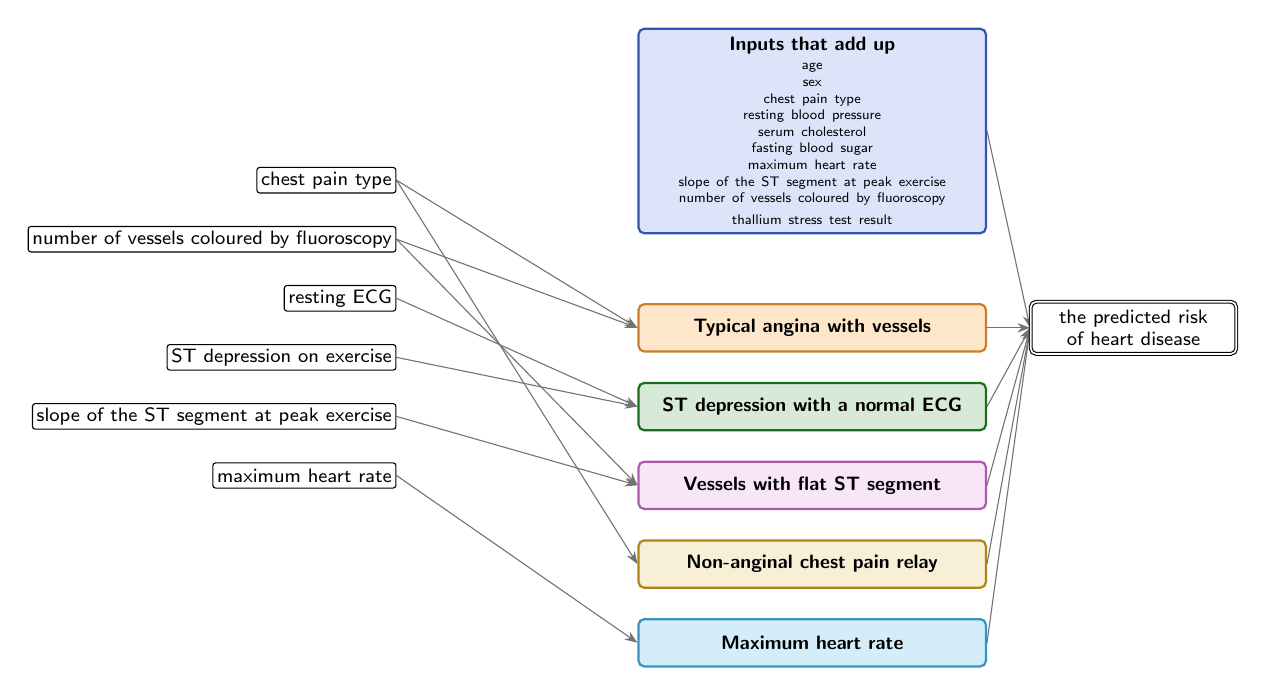
\begin{tikzpicture}[
  font=\sffamily\scriptsize, >={Stealth[length=1.6mm]},
  inp/.style={draw, rounded corners=1pt, fill=white, inner sep=1.5pt, minimum height=3.2mm, anchor=east},
  abox/.style={draw, thick, rounded corners=2pt, align=center, inner sep=3pt, minimum height=6mm, text width=42mm},
  outp/.style={draw, double, rounded corners=2pt, fill=white, align=center, inner sep=3pt, text width=24mm},
  agg/.style={draw=black!55},
]
\node[inp] (i0) at (0,1.875) {chest pain type};
\node[inp] (i1) at (0,1.125) {number of vessels coloured by fluoroscopy};
\node[inp] (i2) at (0,0.375) {resting ECG};
\node[inp] (i3) at (0,-0.375) {ST depression on exercise};
\node[inp] (i4) at (0,-1.125) {slope of the ST segment at peak exercise};
\node[inp] (i5) at (0,-1.875) {maximum heart rate};
\node[abox, fill=RoyalBlue!18, draw=RoyalBlue!80!black] (b0) at (5.28,2.5) {\textbf{Inputs that add up}\\[1pt]{\tiny age\\ sex\\ chest pain type\\ resting blood pressure\\ serum cholesterol\\ fasting blood sugar\\ maximum heart rate\\ slope of the ST segment at peak exercise\\ number of vessels coloured by fluoroscopy\\ thallium stress test result}};
\node[abox, fill=BurntOrange!18, draw=BurntOrange!80!black] (b1) at (5.28,-0.0) {\textbf{Typical angina with vessels}};
\node[abox, fill=ForestGreen!18, draw=ForestGreen!80!black] (b2) at (5.28,-1.0) {\textbf{ST depression with a normal ECG}};
\node[abox, fill=Orchid!18, draw=Orchid!80!black] (b3) at (5.28,-2.0) {\textbf{Vessels with flat ST segment}};
\node[abox, fill=Goldenrod!18, draw=Goldenrod!80!black] (b4) at (5.28,-3.0) {\textbf{Non-anginal chest pain relay}};
\node[abox, fill=Cerulean!18, draw=Cerulean!80!black] (b5) at (5.28,-4.0) {\textbf{Maximum heart rate}};
\node[outp] (out) at (9.36,0) {the predicted risk of heart disease};
\begin{scope}[on background layer]
\draw[->, agg] (b0.east) -- (out.west);
\draw[->, agg, thin] (i0.east) -- (b1.west);
\draw[->, agg, thin] (i1.east) -- (b1.west);
\draw[->, agg] (b1.east) -- (out.west);
\draw[->, agg, thin] (i2.east) -- (b2.west);
\draw[->, agg, thin] (i3.east) -- (b2.west);
\draw[->, agg] (b2.east) -- (out.west);
\draw[->, agg, thin] (i4.east) -- (b3.west);
\draw[->, agg, thin] (i1.east) -- (b3.west);
\draw[->, agg] (b3.east) -- (out.west);
\draw[->, agg, thin] (i0.east) -- (b4.west);
\draw[->, agg] (b4.east) -- (out.west);
\draw[->, agg, thin] (i5.east) -- (b5.west);
\draw[->, agg] (b5.east) -- (out.west);
\end{scope}
\end{tikzpicture}}}%
\caption{The whole model: what feeds it, one level down.}
\label{fig:hearts1c1:parts-ann34}
\end{figure}
\begin{figure}[H]\centering
\resizebox{\ifdim\width>\linewidth\linewidth\else\width\fi}{!}{%
\definecolor{netup}{HTML}{D95F02}\definecolor{netdown}{HTML}{1B9E77}\definecolor{netmixed}{HTML}{7F7F7F}%
\begin{tikzpicture}[
  font=\sffamily\scriptsize, >={Stealth[length=1.4mm]},
  inp/.style={draw, circle, fill=white, minimum size=3.2mm, inner sep=0pt},
  hid/.style={draw, circle, fill=white, minimum size=5.2mm, inner sep=0.5pt, font=\sffamily\tiny},
  exitbox/.style={draw, thick, rectangle, fill=white, align=center, text width=17mm, minimum height=5mm, inner sep=1.5pt, font=\sffamily\tiny},
  sumbox/.style={draw, thick, dashed, rectangle, fill=white, align=center, text width=17mm, minimum height=5mm, inner sep=1.5pt, font=\sffamily\tiny},
  outp/.style={draw, thick, regular polygon, regular polygon sides=6, fill=white, minimum size=10mm, inner sep=0pt, font=\sffamily\tiny, align=center},
  stub/.style={draw, dashed, rounded corners=2pt, fill=white, align=center, inner sep=2pt, font=\sffamily\tiny, text width=15mm},
  inlab/.style={font=\sffamily\tiny, align=center, text width=15mm, inner sep=1pt, fill=white, fill opacity=0.8, text opacity=1},
  wpos/.style={draw=NavyBlue}, wneg/.style={draw=BrickRed}, wagg/.style={draw=black!45, line width=1.2pt},
  wmix/.style={draw=Plum},
]
\node[outp] (n0) at (11.12,3.45) {heart disease};
\node[inp, draw=netup, very thick] (ninxxage) at (0.9,0.0) {};
\path (ninxxage.south) node[inlab, anchor=north] (labninxxage) {age $\uparrow$};
\node[sumbox] (nxxsumxx) at (5.85,1.9) {sum: Inputs that add up};
\node[inp, draw=netdown, very thick] (ninxxsexx0) at (4.5,0.0) {};
\path (ninxxsexx0.south) node[inlab, anchor=north] (labninxxsexx0) {female $\downarrow$};
\node[inp, draw=netdown, very thick] (ninxxcpx2) at (0.9,-2.1) {};
\path (ninxxcpx2.south) node[inlab, anchor=north] (labninxxcpx2) {atypical angina $\downarrow$};
\node[inp, draw=netup, very thick] (ninxxcpx4) at (8.1,0.0) {};
\path (ninxxcpx4.south) node[inlab, anchor=north] (labninxxcpx4) {no chest pain $\uparrow$};
\node[inp, draw=netup, very thick] (ninxxtrestbps) at (1.8,-1.05) {};
\path (ninxxtrestbps.south) node[inlab, anchor=north] (labninxxtrestbps) {blood pressure $\uparrow$};
\node[inp, draw=netup, very thick] (ninxxchol) at (2.7,0.0) {};
\path (ninxxchol.south) node[inlab, anchor=north] (labninxxchol) {cholesterol $\uparrow$};
\node[inp, draw=netdown, very thick] (ninxxfbsx1) at (9.9,0.0) {};
\path (ninxxfbsx1.south) node[inlab, anchor=north] (labninxxfbsx1) {sugar above 120 $\downarrow$};
\node[inp, draw=netup, very thick] (ninxxslopex3) at (3.6,-1.05) {};
\path (ninxxslopex3.south) node[inlab, anchor=north] (labninxxslopex3) {downsloping ST $\uparrow$};
\node[inp, draw=netmixed, very thick] (ninxxthalx3) at (9.0,-1.05) {};
\path (ninxxthalx3.south) node[inlab, anchor=north] (labninxxthalx3) {normal thallium $\updownarrow$};
\node[inp, draw=netdown, very thick] (ninxxthalx6) at (5.4,-1.05) {};
\path (ninxxthalx6.south) node[inlab, anchor=north] (labninxxthalx6) {fixed defect $\downarrow$};
\node[stub] (nfromxxVesselsxwithxflatxSTxsegment) at (21.34,0.0) {from Vessels with flat ST segment};
\node[stub] (nfromxxNonmanginalxchestxpainxrelay) at (15.94,0.0) {from Non-anginal chest pain relay};
\node[stub] (nfromxxSTxdepressionxwithxaxnormalxECG) at (17.74,0.0) {from ST depression with a normal ECG};
\node[stub] (nfromxxMaximumxheartxrate) at (14.14,0.0) {from Maximum heart rate};
\node[stub] (nfromxxTypicalxanginaxwithxvessels) at (19.54,0.0) {from Typical angina with vessels};
\node[inp, draw=netup, very thick] (ninxxca) at (10.8,-1.05) {};
\path (ninxxca.south) node[inlab, anchor=north] (labninxxca) {vessels $\uparrow$};
\node[inp, draw=netup, very thick] (ninxxslopex2) at (6.3,0.0) {};
\path (ninxxslopex2.south) node[inlab, anchor=north] (labninxxslopex2) {flat ST $\uparrow$};
\node[inp, draw=netup, very thick] (ninxxthalach) at (7.2,-1.05) {};
\path (ninxxthalach.south) node[inlab, anchor=north] (labninxxthalach) {max heart rate $\uparrow$};
\begin{scope}[on background layer]
\node[fit=(nxxsumxx) , inner sep=8pt, rounded corners=5pt, fill=RoyalBlue!10, draw=RoyalBlue!45] (clu0) {};
\draw[->, wpos, line width=0.39pt] (ninxxage) -- (nxxsumxx);
\draw[->, wneg, line width=0.90pt] (ninxxsexx0) -- (nxxsumxx);
\draw[->, wpos, line width=0.41pt] (ninxxcpx2) -- (nxxsumxx);
\draw[->, wpos, line width=0.69pt] (ninxxcpx4) -- (nxxsumxx);
\draw[->, wpos, line width=0.48pt] (ninxxtrestbps) -- (nxxsumxx);
\draw[->, wpos, line width=0.58pt] (ninxxchol) -- (nxxsumxx);
\draw[->, wneg, line width=0.36pt] (ninxxfbsx1) -- (nxxsumxx);
\draw[->, wpos, line width=0.32pt] (ninxxslopex3) -- (nxxsumxx);
\draw[->, wneg, line width=0.55pt] (ninxxthalx3) -- (nxxsumxx);
\draw[->, wneg, line width=0.55pt] (ninxxthalx6) -- (nxxsumxx);
\draw[->, wpos, line width=0.57pt] (nfromxxVesselsxwithxflatxSTxsegment) -- (n0);
\draw[->, wneg, line width=0.68pt] (nfromxxNonmanginalxchestxpainxrelay) -- (n0);
\draw[->, wpos, line width=0.74pt] (nfromxxSTxdepressionxwithxaxnormalxECG) -- (n0);
\draw[->, wneg, line width=0.30pt] (nfromxxMaximumxheartxrate) -- (n0);
\draw[->, wpos, line width=0.78pt] (nfromxxTypicalxanginaxwithxvessels) -- (n0);
\draw[->, wneg, line width=0.31pt] (nfromxxMaximumxheartxrate) -- (n0);
\draw[->, wneg, line width=0.54pt] (nfromxxTypicalxanginaxwithxvessels) -- (n0);
\draw[->, wpos, line width=0.70pt] (ninxxca) -- (nxxsumxx);
\draw[->, wpos, line width=0.85pt] (ninxxslopex2) -- (nxxsumxx);
\draw[->, wpos, line width=0.25pt] (ninxxthalach) -- (nxxsumxx);
\draw[->, wagg] (nxxsumxx) -- (n0);
\end{scope}
\node[font=\sffamily\scriptsize\bfseries, text=RoyalBlue!55!black, anchor=south west, inner sep=1pt, fill=white, fill opacity=0.85, text opacity=1] at (clu0.north west) {Inputs that add up};
\end{tikzpicture}}%
\caption{The whole model: its units and every connection into them. Blue: positive weight (raises the score); red: negative weight (lowers it); thicker: larger weight. Orange outline and up arrow: raises the final prediction; teal and down arrow: lowers it; grey and double arrow: depends.}
\label{fig:hearts1c1:units-ann34}
\end{figure}
\paragraph{Hypothesis.} The model adds up its inputs into one score: the vessels coloured (each extra vessel adding about the same), the ST segment, chest pain type and sex each move the predicted risk on their own, five parts add to that sum, and exercise-induced angina is ignored.\,{\scriptsize\textcolor{NavyBlue}{[C29, C01, C02, C10, C28]}}
\paragraph{Evidence.} It is made up of the inputs that feed the score directly and five parts: vessels with a flat ST segment, the non-anginal chest pain relay, ST depression with a normal ECG, the maximum heart rate part and typical angina with vessels (each explained below); the score is their sum, which was checked on all 242 training patients.\,{\scriptsize\textcolor{NavyBlue}{[C29]}} Changing one input at a time across the whole model, each extra vessel adds about the same, taking a typical patient's predicted risk from about 18\% at 0 to about 99\% at 2 vessels, flattening out near the top because the predicted risk cannot go much higher, against about 80\% through the sum alone.\,{\scriptsize\textcolor{NavyBlue}{[C01, C04]}} More ST depression raises it in an uneven way across the whole model, from about 18\% at 0 mm to about 55\% at 2.8 mm; it enters the score only through the part with a normal ECG.\,{\scriptsize\textcolor{NavyBlue}{[C06]}} The model ignores exercise-induced angina.\,{\scriptsize\textcolor{NavyBlue}{[C28]}}
\par\noindent{\small Evidence plots: Figure~\ref{fig:hearts1c1:plot-ann34-0}.\par}
\begin{figure}[H]\centering
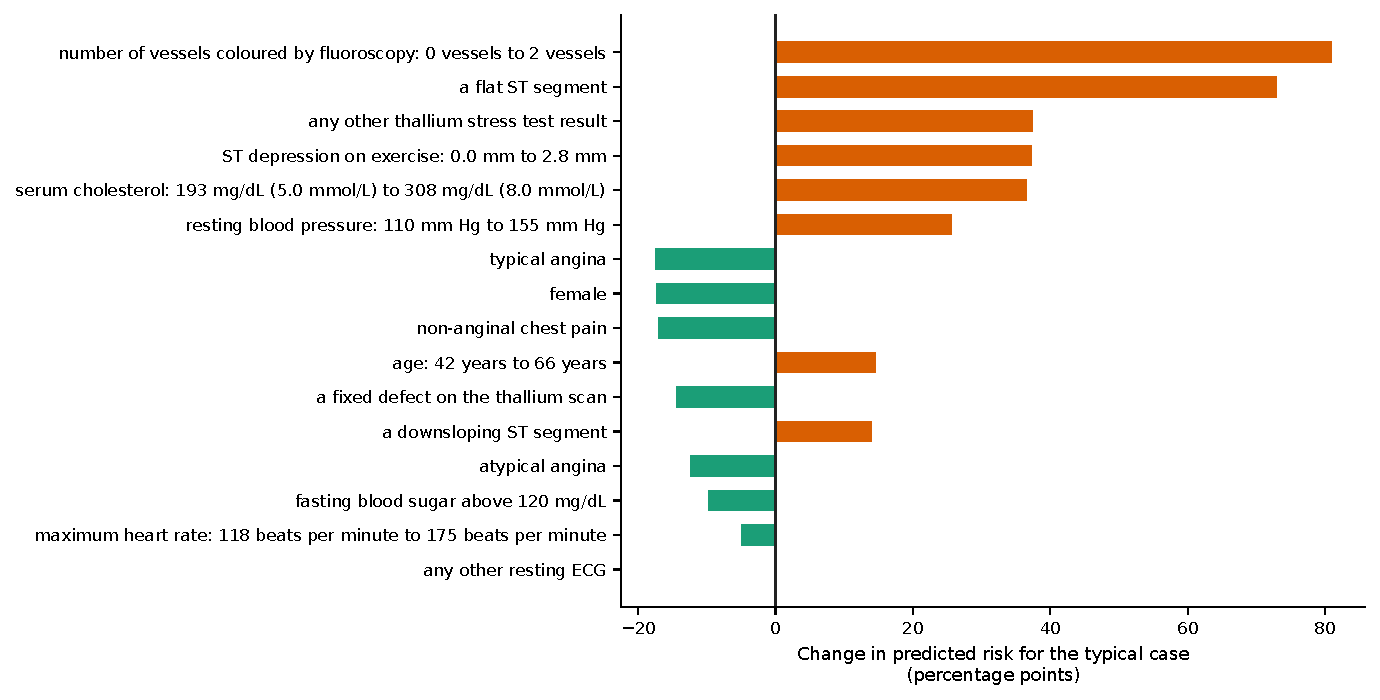
\includegraphics[width=\linewidth,height=0.88\textheight,keepaspectratio]{figures/heart-s1-c1/ann_34-effects.pdf}
\caption{The whole model: Each input's change in the predicted value for the typical case across the whole model, largest first (orange: raises it, teal: lowers it).}
\label{fig:hearts1c1:plot-ann34-0}
\end{figure}
\par\smallskip\noindent{\small \textbf{Dive deeper:} Typical angina with vessels (\ref{rd:ann33}); ST depression with a normal ECG (\ref{rd:ann31}); Vessels with flat ST segment (\ref{rd:ann29}); Non-anginal chest pain relay (\ref{rd:ann30}); Maximum heart rate (\ref{rd:ann32}). Technical detail: \ref{tech:ann34}.\par}
\subsubsection{Typical angina with vessels}\label{rd:ann33}
\noindent{\footnotesize Part of: The whole model (\ref{rd:ann34}).\par}
\noindent{\small Figure~\ref{fig:hearts1c1:parts-ann33} shows what feeds this part; Figure~\ref{fig:hearts1c1:units-ann33} its units and every connection into them (dashed boxes: connections from or to other parts, drawn in their own sections).\par}
\begin{figure}[H]\centering
\resizebox{!}{\ifdim\height>0.5\textheight 0.5\textheight\else\height\fi}{%
\resizebox{\ifdim\width>\linewidth\linewidth\else\width\fi}{!}{%
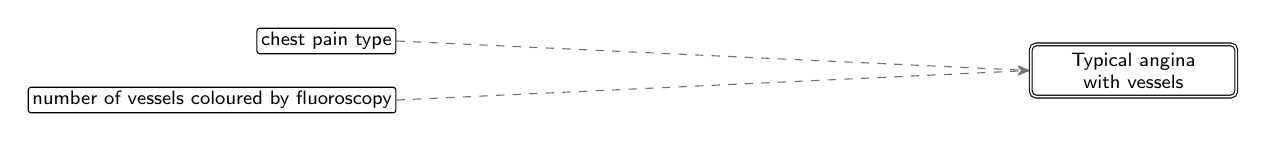
\begin{tikzpicture}[
  font=\sffamily\scriptsize, >={Stealth[length=1.6mm]},
  inp/.style={draw, rounded corners=1pt, fill=white, inner sep=1.5pt, minimum height=3.2mm, anchor=east},
  abox/.style={draw, thick, rounded corners=2pt, align=center, inner sep=3pt, minimum height=6mm, text width=42mm},
  outp/.style={draw, double, rounded corners=2pt, fill=white, align=center, inner sep=3pt, text width=24mm},
  agg/.style={draw=black!55},
]
\node[inp] (i0) at (0,0.375) {chest pain type};
\node[inp] (i1) at (0,-0.375) {number of vessels coloured by fluoroscopy};
\node[outp] (out) at (9.36,0) {Typical angina with vessels};
\begin{scope}[on background layer]
\draw[->, agg, thin, dashed] (i0.east) -- (out.west);
\draw[->, agg, thin, dashed] (i1.east) -- (out.west);
\end{scope}
\end{tikzpicture}}}%
\caption{Typical angina with vessels: what feeds it, one level down.}
\label{fig:hearts1c1:parts-ann33}
\end{figure}
\begin{figure}[H]\centering
\resizebox{\ifdim\width>\linewidth\linewidth\else\width\fi}{!}{%
\definecolor{netup}{HTML}{D95F02}\definecolor{netdown}{HTML}{1B9E77}\definecolor{netmixed}{HTML}{7F7F7F}%
\begin{tikzpicture}[
  font=\sffamily\scriptsize, >={Stealth[length=1.4mm]},
  inp/.style={draw, circle, fill=white, minimum size=3.2mm, inner sep=0pt},
  hid/.style={draw, circle, fill=white, minimum size=5.2mm, inner sep=0.5pt, font=\sffamily\tiny},
  exitbox/.style={draw, thick, rectangle, fill=white, align=center, text width=17mm, minimum height=5mm, inner sep=1.5pt, font=\sffamily\tiny},
  sumbox/.style={draw, thick, dashed, rectangle, fill=white, align=center, text width=17mm, minimum height=5mm, inner sep=1.5pt, font=\sffamily\tiny},
  outp/.style={draw, thick, regular polygon, regular polygon sides=6, fill=white, minimum size=10mm, inner sep=0pt, font=\sffamily\tiny, align=center},
  stub/.style={draw, dashed, rounded corners=2pt, fill=white, align=center, inner sep=2pt, font=\sffamily\tiny, text width=15mm},
  inlab/.style={font=\sffamily\tiny, align=center, text width=15mm, inner sep=1pt, fill=white, fill opacity=0.8, text opacity=1},
  wpos/.style={draw=NavyBlue}, wneg/.style={draw=BrickRed}, wagg/.style={draw=black!45, line width=1.2pt},
  wmix/.style={draw=Plum},
]
\node[hid] (n2245) at (2.7,1.9) {h5};
\node[hid] (n3210) at (2.7,3.25) {h7};
\node[inp, draw=netdown, very thick] (ninxxcpx1) at (1.8,0.0) {};
\path (ninxxcpx1.south) node[inlab, anchor=north] (labninxxcpx1) {typical angina $\downarrow$};
\node[inp, draw=netup, very thick] (ninxxca) at (3.6,0.0) {};
\path (ninxxca.south) node[inlab, anchor=north] (labninxxca) {vessels $\uparrow$};
\node[stub] (ntoxxthexmodelxoutput) at (2.7,4.8) {to the model output};
\begin{scope}[on background layer]
\node[fit=(n2245) (n3210) , inner sep=8pt, rounded corners=5pt, fill=BurntOrange!10, draw=BurntOrange!45] (clu0) {};
\draw[->, wpos, line width=0.57pt] (ninxxcpx1) -- (n3210);
\draw[->, wneg, line width=0.48pt] (n2245) -- (n3210);
\draw[->, wpos, line width=0.45pt] (ninxxca) -- (n2245);
\draw[->, wpos, line width=0.78pt] (n2245) -- (ntoxxthexmodelxoutput);
\draw[->, wneg, line width=0.54pt] (n3210) -- (ntoxxthexmodelxoutput);
\end{scope}
\node[font=\sffamily\scriptsize\bfseries, text=BurntOrange!55!black, anchor=south west, inner sep=1pt, fill=white, fill opacity=0.85, text opacity=1] at (clu0.north west) {Typical angina with vessels};
\end{tikzpicture}}%
\caption{Typical angina with vessels: its units and every connection into them. Blue: positive weight (raises the score); red: negative weight (lowers it); thicker: larger weight. Orange outline and up arrow: raises the final prediction; teal and down arrow: lowers it; grey and double arrow: depends.}
\label{fig:hearts1c1:units-ann33}
\end{figure}
\paragraph{Hypothesis.} This part lowers the predicted risk for typical angina and adds risk for each extra vessel coloured, about the same for each, with the vessels counting more for patients with typical angina.\,{\scriptsize\textcolor{NavyBlue}{[C31, C30, C32]}}
\paragraph{Evidence.} Through it, typical angina takes a typical patient's predicted risk from about 18\% to about 2\%, and each extra vessel adds about the same, from about 18\% at 0 to about 61\% at 2 vessels.\,{\scriptsize\textcolor{NavyBlue}{[C31, C30]}} Across the whole model, going from 0 to 2 vessels moves a typical patient from below 1\% to about 55\% with typical angina, each extra vessel adding about the same, and from about 18\% to about 99\% with any other chest pain type.\,{\scriptsize\textcolor{NavyBlue}{[C32]}} Its formula reproduces the part exactly on all 242 training patients.\,{\scriptsize\textcolor{NavyBlue}{[C33]}}
\par\noindent{\small Evidence plots: Figure~\ref{fig:hearts1c1:plot-ann33-0}, Figure~\ref{fig:hearts1c1:plot-ann33-1}, Figure~\ref{fig:hearts1c1:plot-ann33-2}, Figure~\ref{fig:hearts1c1:plot-ann33-3}, Figure~\ref{fig:hearts1c1:plot-ann33-4}, Figure~\ref{fig:hearts1c1:plot-ann33-5}.\par}
\par\noindent{\small Figure~\ref{fig:hearts1c1:plot-ann33-3} shows this part's own output, unit h5.\par}
\par\noindent{\small Figure~\ref{fig:hearts1c1:plot-ann33-4} shows this part's own output, unit h7.\par}
\begin{figure}[H]\centering
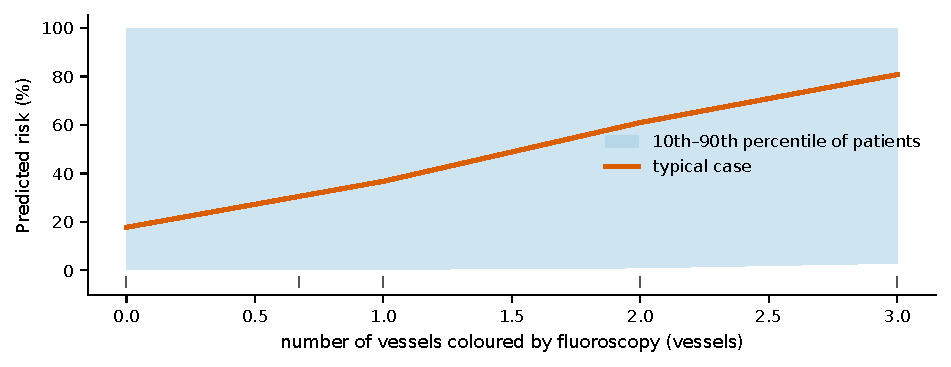
\includegraphics[width=\linewidth,height=0.88\textheight,keepaspectratio]{figures/heart-s1-c1/ann_33-response.pdf}
\caption{Typical angina with vessels: Response curves through this part: the typical case (bold), the 10th to 90th percentile of individual patients (band), the fold or step point (dashed) with its spread across them (grey), and the observed values (ticks).}
\label{fig:hearts1c1:plot-ann33-0}
\end{figure}
\begin{figure}[H]\centering
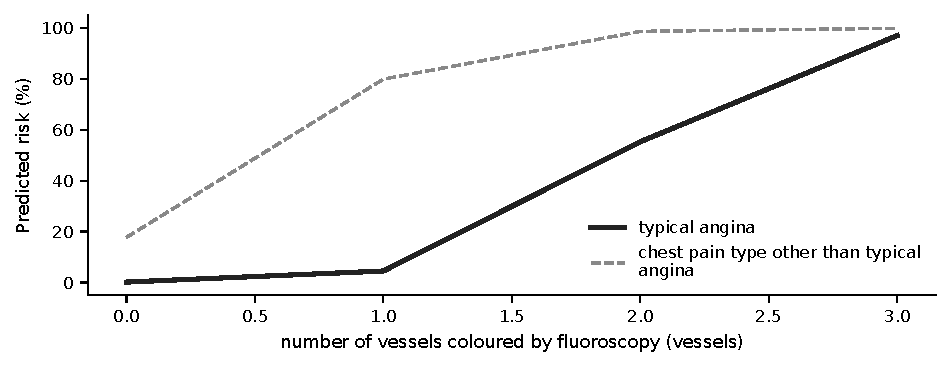
\includegraphics[width=\linewidth,height=0.88\textheight,keepaspectratio]{figures/heart-s1-c1/ann_33-interaction.pdf}
\caption{Typical angina with vessels: How the effect differs between groups: one curve per group, for the typical case of each group.}
\label{fig:hearts1c1:plot-ann33-1}
\end{figure}
\begin{figure}[H]\centering
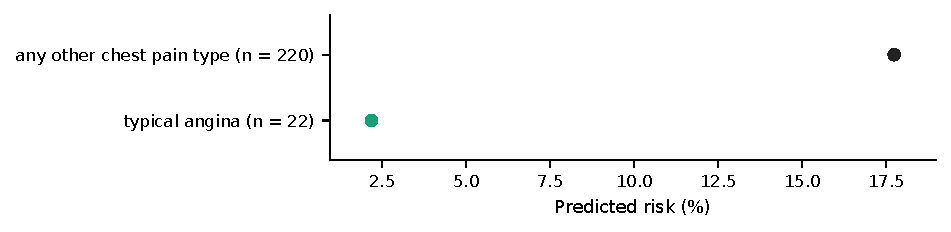
\includegraphics[width=\linewidth,height=0.88\textheight,keepaspectratio]{figures/heart-s1-c1/ann_33-categories-small.pdf}
\caption{Typical angina with vessels: The predicted value for the typical case at each level, through this part (n = training patients; grey: fewer than 20).}
\label{fig:hearts1c1:plot-ann33-2}
\end{figure}
\begin{figure}[H]\centering
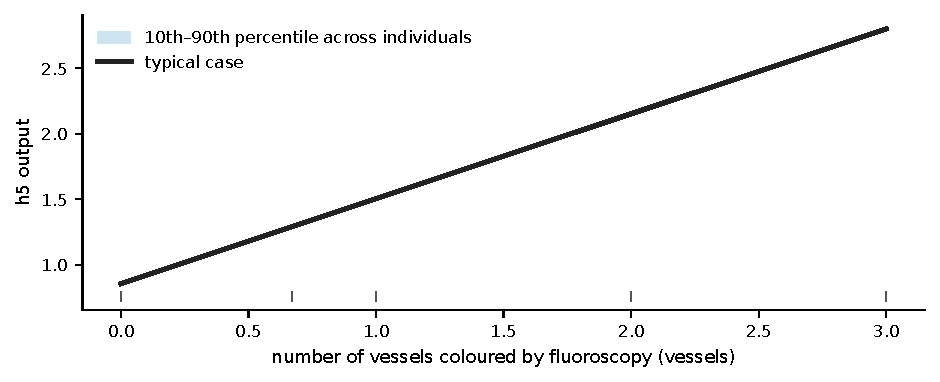
\includegraphics[width=\linewidth,height=0.88\textheight,keepaspectratio]{figures/heart-s1-c1/ann_33-partial-2245.pdf}
\caption{Typical angina with vessels: This part's own output, unit h5 (the output of 'Typical angina with vessels'), on its own scale (its activation), with every other input at the typical case; it is active for 242 of 242. Bold: the typical case; band: 10th to 90th percentile across individuals; ticks: the data.}
\label{fig:hearts1c1:plot-ann33-3}
\end{figure}
\begin{figure}[H]\centering
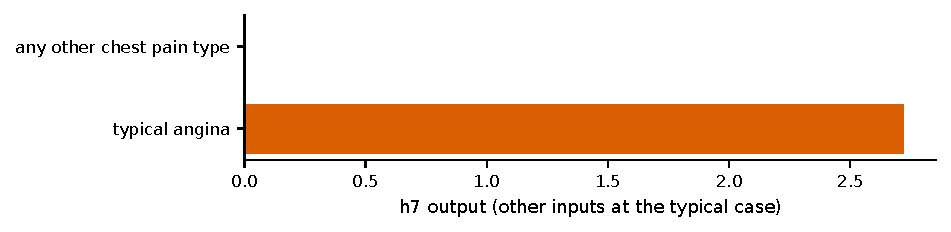
\includegraphics[width=\linewidth,height=0.88\textheight,keepaspectratio]{figures/heart-s1-c1/ann_33-partial-3210.pdf}
\caption{Typical angina with vessels: This part's own output, unit h7 (the output of 'Typical angina with vessels'), on its own scale (its activation), with every other input at the typical case; it is active for 22 of 242. Its output for each combination of the levels it reads.}
\label{fig:hearts1c1:plot-ann33-4}
\end{figure}
\begin{figure}[H]\centering
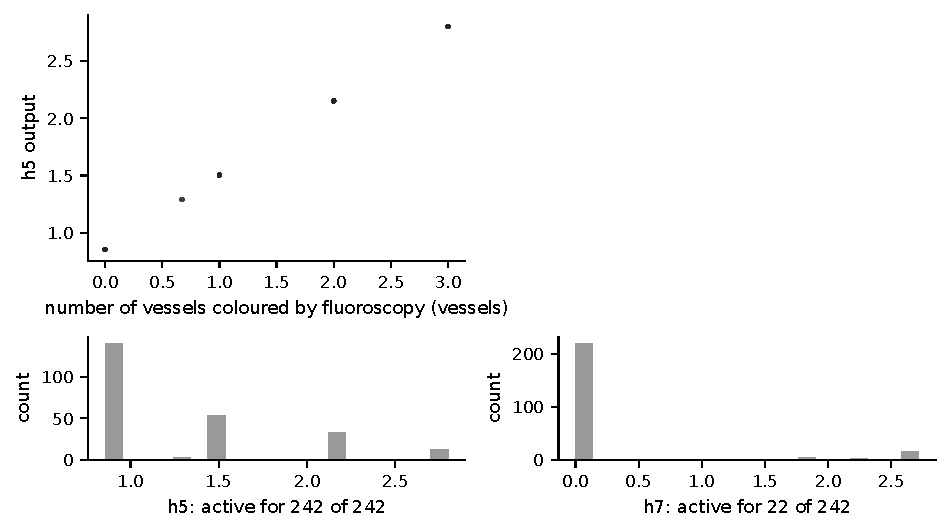
\includegraphics[width=\linewidth,height=0.88\textheight,keepaspectratio]{figures/heart-s1-c1/ann_33-units.pdf}
\caption{Typical angina with vessels: This part's hidden units: each unit's output against its main numeric input (top) and how often it is active (bottom).}
\label{fig:hearts1c1:plot-ann33-5}
\end{figure}
\par\smallskip\noindent{\small Technical detail: \ref{tech:ann33}.\par}
\subsubsection{ST depression with a normal ECG}\label{rd:ann31}
\noindent{\footnotesize Part of: The whole model (\ref{rd:ann34}).\par}
\noindent{\small Figure~\ref{fig:hearts1c1:parts-ann31} shows what feeds this part; Figure~\ref{fig:hearts1c1:units-ann31} its units and every connection into them (dashed boxes: connections from or to other parts, drawn in their own sections).\par}
\begin{figure}[H]\centering
\resizebox{!}{\ifdim\height>0.5\textheight 0.5\textheight\else\height\fi}{%
\resizebox{\ifdim\width>\linewidth\linewidth\else\width\fi}{!}{%
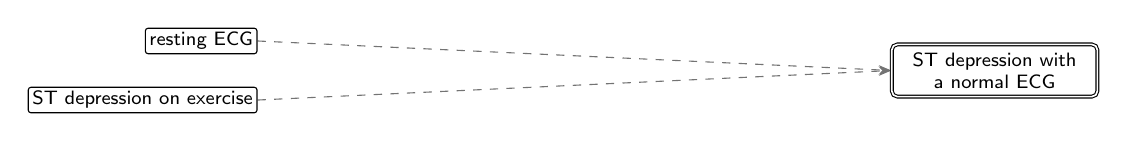
\begin{tikzpicture}[
  font=\sffamily\scriptsize, >={Stealth[length=1.6mm]},
  inp/.style={draw, rounded corners=1pt, fill=white, inner sep=1.5pt, minimum height=3.2mm, anchor=east},
  abox/.style={draw, thick, rounded corners=2pt, align=center, inner sep=3pt, minimum height=6mm, text width=42mm},
  outp/.style={draw, double, rounded corners=2pt, fill=white, align=center, inner sep=3pt, text width=24mm},
  agg/.style={draw=black!55},
]
\node[inp] (i0) at (0,0.375) {resting ECG};
\node[inp] (i1) at (0,-0.375) {ST depression on exercise};
\node[outp] (out) at (9.36,0) {ST depression with a normal ECG};
\begin{scope}[on background layer]
\draw[->, agg, thin, dashed] (i0.east) -- (out.west);
\draw[->, agg, thin, dashed] (i1.east) -- (out.west);
\end{scope}
\end{tikzpicture}}}%
\caption{ST depression with a normal ECG: what feeds it, one level down.}
\label{fig:hearts1c1:parts-ann31}
\end{figure}
\begin{figure}[H]\centering
\resizebox{\ifdim\width>\linewidth\linewidth\else\width\fi}{!}{%
\definecolor{netup}{HTML}{D95F02}\definecolor{netdown}{HTML}{1B9E77}\definecolor{netmixed}{HTML}{7F7F7F}%
\begin{tikzpicture}[
  font=\sffamily\scriptsize, >={Stealth[length=1.4mm]},
  inp/.style={draw, circle, fill=white, minimum size=3.2mm, inner sep=0pt},
  hid/.style={draw, circle, fill=white, minimum size=5.2mm, inner sep=0.5pt, font=\sffamily\tiny},
  exitbox/.style={draw, thick, rectangle, fill=white, align=center, text width=17mm, minimum height=5mm, inner sep=1.5pt, font=\sffamily\tiny},
  sumbox/.style={draw, thick, dashed, rectangle, fill=white, align=center, text width=17mm, minimum height=5mm, inner sep=1.5pt, font=\sffamily\tiny},
  outp/.style={draw, thick, regular polygon, regular polygon sides=6, fill=white, minimum size=10mm, inner sep=0pt, font=\sffamily\tiny, align=center},
  stub/.style={draw, dashed, rounded corners=2pt, fill=white, align=center, inner sep=2pt, font=\sffamily\tiny, text width=15mm},
  inlab/.style={font=\sffamily\tiny, align=center, text width=15mm, inner sep=1pt, fill=white, fill opacity=0.8, text opacity=1},
  wpos/.style={draw=NavyBlue}, wneg/.style={draw=BrickRed}, wagg/.style={draw=black!45, line width=1.2pt},
  wmix/.style={draw=Plum},
]
\node[exitbox] (n1801) at (3.1,1.9) {ST depression with a normal ECG $\uparrow$};
\node[inp, draw=netup, very thick] (ninxxrestecgx0) at (4.0,0.0) {};
\path (ninxxrestecgx0.south) node[inlab, anchor=north] (labninxxrestecgx0) {normal ECG $\uparrow$};
\node[inp, draw=netup, very thick] (ninxxoldpeak) at (2.2,0.0) {};
\path (ninxxoldpeak.south) node[inlab, anchor=north] (labninxxoldpeak) {ST depression $\uparrow$};
\node[stub] (ntoxxthexmodelxoutput) at (3.1,3.45) {to the model output};
\begin{scope}[on background layer]
\node[fit=(n1801) , inner sep=8pt, rounded corners=5pt, fill=ForestGreen!10, draw=ForestGreen!45] (clu0) {};
\draw[->, wpos, line width=0.79pt] (ninxxrestecgx0) -- (n1801);
\draw[->, wpos, line width=0.54pt] (ninxxoldpeak) -- (n1801);
\draw[->, wpos, line width=0.74pt] (n1801) -- (ntoxxthexmodelxoutput);
\end{scope}
\node[font=\sffamily\scriptsize\bfseries, text=ForestGreen!55!black, anchor=south west, inner sep=1pt, fill=white, fill opacity=0.85, text opacity=1] at (clu0.north west) {ST depression with a normal ECG};
\end{tikzpicture}}%
\caption{ST depression with a normal ECG: its units and every connection into them. Blue: positive weight (raises the score); red: negative weight (lowers it); thicker: larger weight. Orange outline and up arrow: raises the final prediction; teal and down arrow: lowers it; grey and double arrow: depends.}
\label{fig:hearts1c1:units-ann31}
\end{figure}
\paragraph{Hypothesis.} This part raises the predicted risk with ST depression on exercise, in an uneven way, only for patients with a normal resting ECG, once it rises above about 1.0 mm.\,{\scriptsize\textcolor{NavyBlue}{[C37, C36]}}
\paragraph{Evidence.} It acts on 42 of 242 training patients, nearly all with a normal resting ECG, 26 of whom had heart disease; for the typical patient it acts on, the predicted risk is about 98\% without it and about 99\% with it.\,{\scriptsize\textcolor{NavyBlue}{[C38]}} Through it, more ST depression raises the predicted risk only once it rises above about 1.0 mm, in an uneven way: for a typical patient with a normal resting ECG from about 13\% at 0 mm to about 63\% at 3.5 mm.\,{\scriptsize\textcolor{NavyBlue}{[C37]}} Going from 0 to 2.8 mm of ST depression moves a typical patient from about 18\% to about 55\% with a normal resting ECG, in an uneven way, and leaves it at about 18\% otherwise.\,{\scriptsize\textcolor{NavyBlue}{[C36]}} Its formula reproduces the part exactly on all 242 training patients.\,{\scriptsize\textcolor{NavyBlue}{[C39]}}
\par\noindent{\small Evidence plots: Figure~\ref{fig:hearts1c1:plot-ann31-0}, Figure~\ref{fig:hearts1c1:plot-ann31-1}, Figure~\ref{fig:hearts1c1:plot-ann31-2}, Figure~\ref{fig:hearts1c1:plot-ann31-3}, Figure~\ref{fig:hearts1c1:plot-ann31-4}.\par}
\par\noindent{\small Figure~\ref{fig:hearts1c1:plot-ann31-3} shows this part's own output, unit h3: it switches on at about 1.006 mm of ST depression on exercise, and is zero below.\par}
\begin{figure}[H]\centering
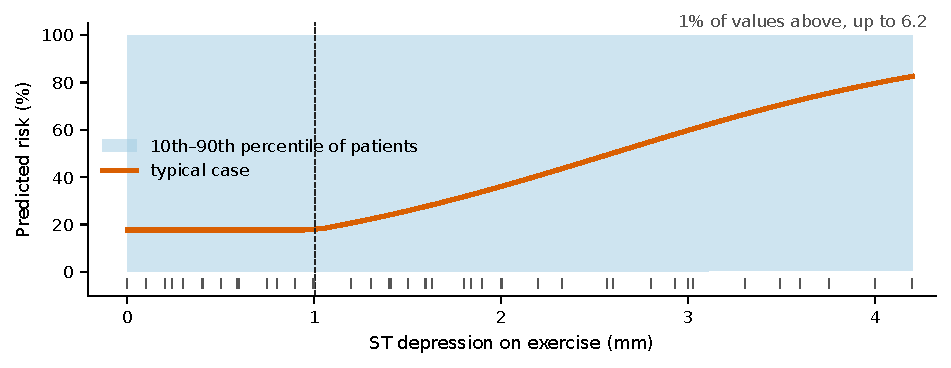
\includegraphics[width=\linewidth,height=0.88\textheight,keepaspectratio]{figures/heart-s1-c1/ann_31-response.pdf}
\caption{ST depression with a normal ECG: Response curves through this part: the typical case (bold), the 10th to 90th percentile of individual patients (band), the fold or step point (dashed) with its spread across them (grey), and the observed values (ticks).}
\label{fig:hearts1c1:plot-ann31-0}
\end{figure}
\begin{figure}[H]\centering
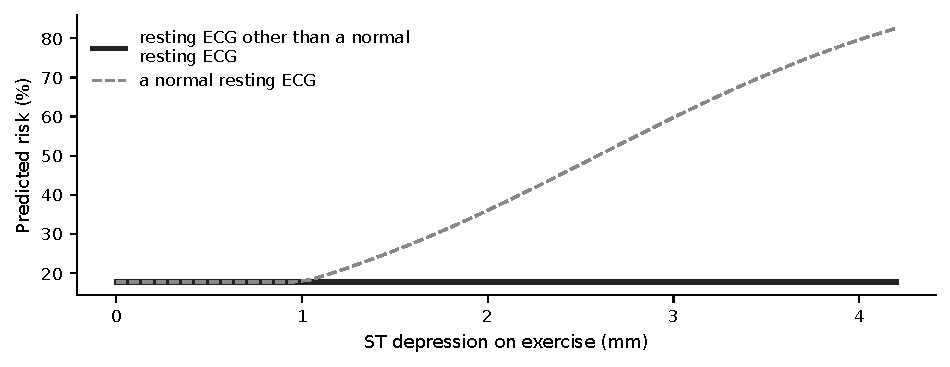
\includegraphics[width=\linewidth,height=0.88\textheight,keepaspectratio]{figures/heart-s1-c1/ann_31-interaction.pdf}
\caption{ST depression with a normal ECG: How the effect differs between groups: one curve per group, for the typical case of each group.}
\label{fig:hearts1c1:plot-ann31-1}
\end{figure}
\begin{figure}[H]\centering
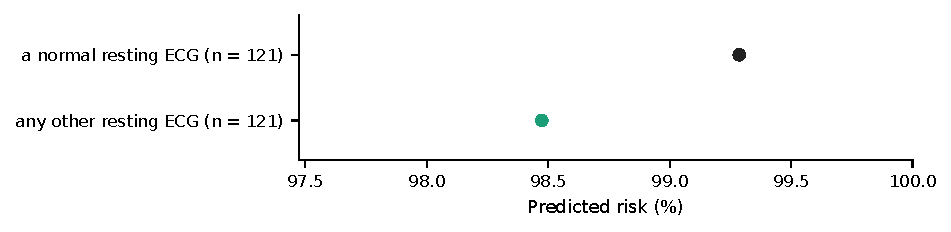
\includegraphics[width=\linewidth,height=0.88\textheight,keepaspectratio]{figures/heart-s1-c1/ann_31-categories-small.pdf}
\caption{ST depression with a normal ECG: The predicted value for the typical case at each level, through this part (n = training patients; grey: fewer than 20).}
\label{fig:hearts1c1:plot-ann31-2}
\end{figure}
\begin{figure}[H]\centering
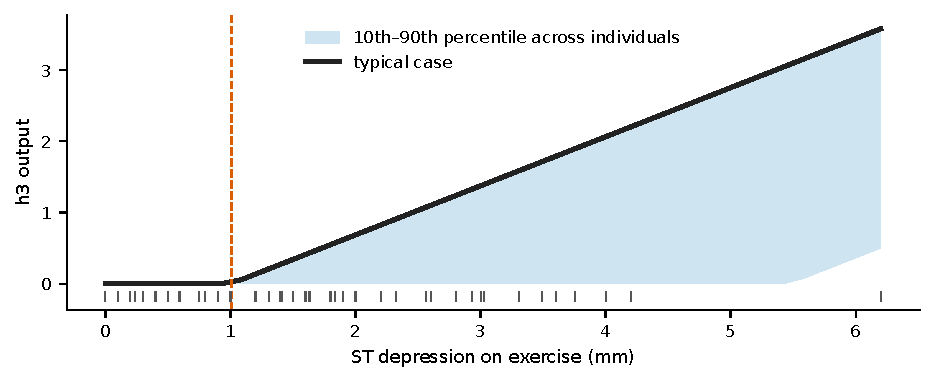
\includegraphics[width=\linewidth,height=0.88\textheight,keepaspectratio]{figures/heart-s1-c1/ann_31-partial-1801.pdf}
\caption{ST depression with a normal ECG: This part's own output, unit h3 (the output of 'ST depression with a normal ECG'), on its own scale (its activation), with every other input at the typical case; it is active for 42 of 242. Bold: the typical case; band: 10th to 90th percentile across individuals; dashed: where it switches on; ticks: the data.}
\label{fig:hearts1c1:plot-ann31-3}
\end{figure}
\begin{figure}[H]\centering
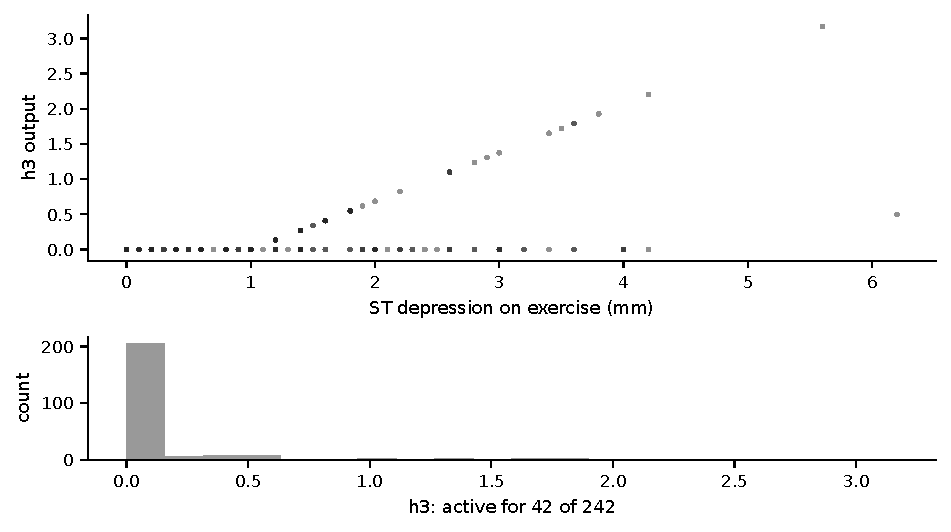
\includegraphics[width=\linewidth,height=0.88\textheight,keepaspectratio]{figures/heart-s1-c1/ann_31-units.pdf}
\caption{ST depression with a normal ECG: This part's hidden units: each unit's output against its main numeric input (top) and how often it is active (bottom).}
\label{fig:hearts1c1:plot-ann31-4}
\end{figure}
\par\smallskip\noindent{\small Technical detail: \ref{tech:ann31}.\par}
\subsubsection{Vessels with flat ST segment}\label{rd:ann29}
\noindent{\footnotesize Part of: The whole model (\ref{rd:ann34}).\par}
\noindent{\small Figure~\ref{fig:hearts1c1:parts-ann29} shows what feeds this part; Figure~\ref{fig:hearts1c1:units-ann29} its units and every connection into them (dashed boxes: connections from or to other parts, drawn in their own sections).\par}
\begin{figure}[H]\centering
\resizebox{!}{\ifdim\height>0.5\textheight 0.5\textheight\else\height\fi}{%
\resizebox{\ifdim\width>\linewidth\linewidth\else\width\fi}{!}{%
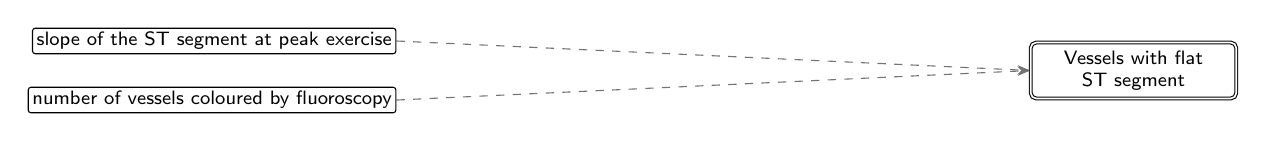
\begin{tikzpicture}[
  font=\sffamily\scriptsize, >={Stealth[length=1.6mm]},
  inp/.style={draw, rounded corners=1pt, fill=white, inner sep=1.5pt, minimum height=3.2mm, anchor=east},
  abox/.style={draw, thick, rounded corners=2pt, align=center, inner sep=3pt, minimum height=6mm, text width=42mm},
  outp/.style={draw, double, rounded corners=2pt, fill=white, align=center, inner sep=3pt, text width=24mm},
  agg/.style={draw=black!55},
]
\node[inp] (i0) at (0,0.375) {slope of the ST segment at peak exercise};
\node[inp] (i1) at (0,-0.375) {number of vessels coloured by fluoroscopy};
\node[outp] (out) at (9.36,0) {Vessels with flat ST segment};
\begin{scope}[on background layer]
\draw[->, agg, thin, dashed] (i0.east) -- (out.west);
\draw[->, agg, thin, dashed] (i1.east) -- (out.west);
\end{scope}
\end{tikzpicture}}}%
\caption{Vessels with flat ST segment: what feeds it, one level down.}
\label{fig:hearts1c1:parts-ann29}
\end{figure}
\begin{figure}[H]\centering
\resizebox{\ifdim\width>\linewidth\linewidth\else\width\fi}{!}{%
\definecolor{netup}{HTML}{D95F02}\definecolor{netdown}{HTML}{1B9E77}\definecolor{netmixed}{HTML}{7F7F7F}%
\begin{tikzpicture}[
  font=\sffamily\scriptsize, >={Stealth[length=1.4mm]},
  inp/.style={draw, circle, fill=white, minimum size=3.2mm, inner sep=0pt},
  hid/.style={draw, circle, fill=white, minimum size=5.2mm, inner sep=0.5pt, font=\sffamily\tiny},
  exitbox/.style={draw, thick, rectangle, fill=white, align=center, text width=17mm, minimum height=5mm, inner sep=1.5pt, font=\sffamily\tiny},
  sumbox/.style={draw, thick, dashed, rectangle, fill=white, align=center, text width=17mm, minimum height=5mm, inner sep=1.5pt, font=\sffamily\tiny},
  outp/.style={draw, thick, regular polygon, regular polygon sides=6, fill=white, minimum size=10mm, inner sep=0pt, font=\sffamily\tiny, align=center},
  stub/.style={draw, dashed, rounded corners=2pt, fill=white, align=center, inner sep=2pt, font=\sffamily\tiny, text width=15mm},
  inlab/.style={font=\sffamily\tiny, align=center, text width=15mm, inner sep=1pt, fill=white, fill opacity=0.8, text opacity=1},
  wpos/.style={draw=NavyBlue}, wneg/.style={draw=BrickRed}, wagg/.style={draw=black!45, line width=1.2pt},
  wmix/.style={draw=Plum},
]
\node[exitbox] (n664) at (2.8,1.9) {Vessels with flat ST segment $\uparrow$};
\node[inp, draw=netup, very thick] (ninxxca) at (3.7,0.0) {};
\path (ninxxca.south) node[inlab, anchor=north] (labninxxca) {vessels $\uparrow$};
\node[inp, draw=netup, very thick] (ninxxslopex2) at (1.9,0.0) {};
\path (ninxxslopex2.south) node[inlab, anchor=north] (labninxxslopex2) {flat ST $\uparrow$};
\node[stub] (ntoxxthexmodelxoutput) at (2.8,3.45) {to the model output};
\begin{scope}[on background layer]
\node[fit=(n664) , inner sep=8pt, rounded corners=5pt, fill=Orchid!10, draw=Orchid!45] (clu0) {};
\draw[->, wpos, line width=0.41pt] (ninxxca) -- (n664);
\draw[->, wpos, line width=0.31pt] (ninxxslopex2) -- (n664);
\draw[->, wpos, line width=0.57pt] (n664) -- (ntoxxthexmodelxoutput);
\end{scope}
\node[font=\sffamily\scriptsize\bfseries, text=Orchid!55!black, anchor=south west, inner sep=1pt, fill=white, fill opacity=0.85, text opacity=1] at (clu0.north west) {Vessels with flat ST segment};
\end{tikzpicture}}%
\caption{Vessels with flat ST segment: its units and every connection into them. Blue: positive weight (raises the score); red: negative weight (lowers it); thicker: larger weight. Orange outline and up arrow: raises the final prediction; teal and down arrow: lowers it; grey and double arrow: depends.}
\label{fig:hearts1c1:units-ann29}
\end{figure}
\paragraph{Hypothesis.} This part adds risk for each extra vessel coloured, about the same for each, and for a flat ST segment.\,{\scriptsize\textcolor{NavyBlue}{[C40, C41]}}
\paragraph{Evidence.} Through it, each extra vessel adds about the same, from about 18\% at 0 to about 36\% at 2 vessels for a typical patient, and a flat ST segment raises the risk from about 18\% to about 23\%.\,{\scriptsize\textcolor{NavyBlue}{[C40, C41]}} Its formula reproduces the part exactly on all 242 training patients.\,{\scriptsize\textcolor{NavyBlue}{[C42]}}
\par\noindent{\small Evidence plots: Figure~\ref{fig:hearts1c1:plot-ann29-0}, Figure~\ref{fig:hearts1c1:plot-ann29-1}, Figure~\ref{fig:hearts1c1:plot-ann29-2}.\par}
\begin{figure}[H]\centering
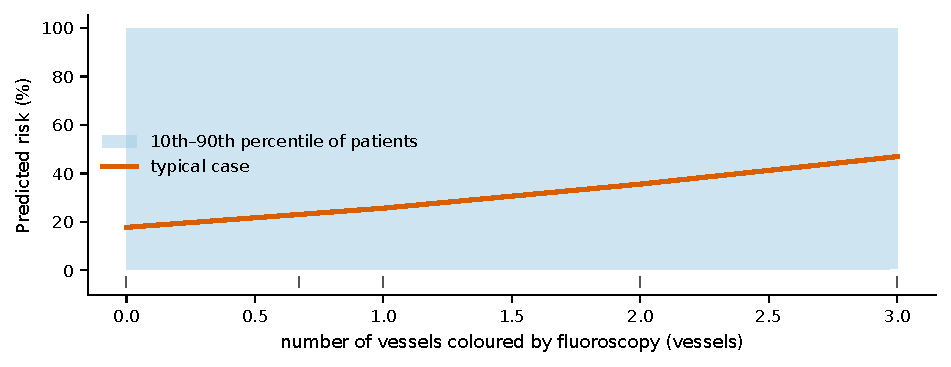
\includegraphics[width=\linewidth,height=0.88\textheight,keepaspectratio]{figures/heart-s1-c1/ann_29-response.pdf}
\caption{Vessels with flat ST segment: Response curves through this part: the typical case (bold), the 10th to 90th percentile of individual patients (band), the fold or step point (dashed) with its spread across them (grey), and the observed values (ticks).}
\label{fig:hearts1c1:plot-ann29-0}
\end{figure}
\begin{figure}[H]\centering
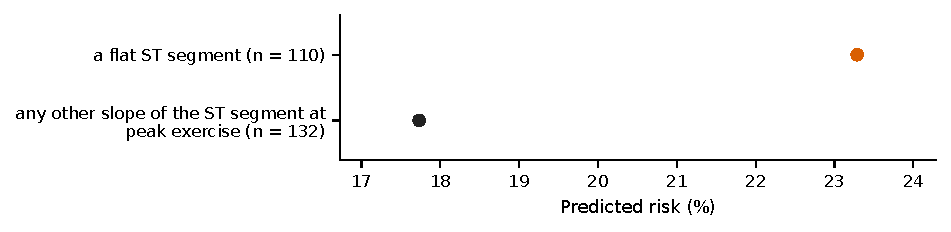
\includegraphics[width=\linewidth,height=0.88\textheight,keepaspectratio]{figures/heart-s1-c1/ann_29-categories-small.pdf}
\caption{Vessels with flat ST segment: The predicted value for the typical case at each level, through this part (n = training patients; grey: fewer than 20).}
\label{fig:hearts1c1:plot-ann29-1}
\end{figure}
\begin{figure}[H]\centering
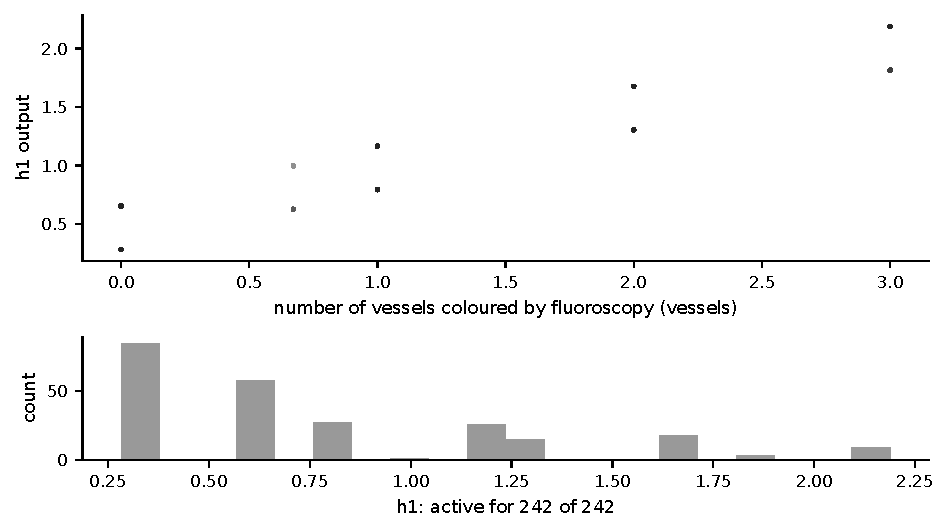
\includegraphics[width=\linewidth,height=0.88\textheight,keepaspectratio]{figures/heart-s1-c1/ann_29-units.pdf}
\caption{Vessels with flat ST segment: This part's hidden units: each unit's output against its main numeric input (top) and how often it is active (bottom).}
\label{fig:hearts1c1:plot-ann29-2}
\end{figure}
\par\smallskip\noindent{\small Technical detail: \ref{tech:ann29}.\par}
\subsubsection{Non-anginal chest pain relay}\label{rd:ann30}
\noindent{\footnotesize Part of: The whole model (\ref{rd:ann34}).\par}
\noindent{\small Figure~\ref{fig:hearts1c1:parts-ann30} shows what feeds this part; Figure~\ref{fig:hearts1c1:units-ann30} its units and every connection into them (dashed boxes: connections from or to other parts, drawn in their own sections).\par}
\begin{figure}[H]\centering
\resizebox{!}{\ifdim\height>0.5\textheight 0.5\textheight\else\height\fi}{%
\resizebox{\ifdim\width>\linewidth\linewidth\else\width\fi}{!}{%
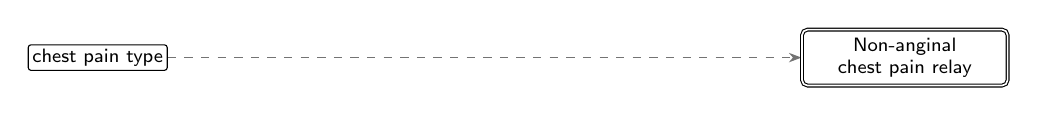
\begin{tikzpicture}[
  font=\sffamily\scriptsize, >={Stealth[length=1.6mm]},
  inp/.style={draw, rounded corners=1pt, fill=white, inner sep=1.5pt, minimum height=3.2mm, anchor=east},
  abox/.style={draw, thick, rounded corners=2pt, align=center, inner sep=3pt, minimum height=6mm, text width=42mm},
  outp/.style={draw, double, rounded corners=2pt, fill=white, align=center, inner sep=3pt, text width=24mm},
  agg/.style={draw=black!55},
]
\node[inp] (i0) at (0,-0.0) {chest pain type};
\node[outp] (out) at (9.36,0) {Non-anginal chest pain relay};
\begin{scope}[on background layer]
\draw[->, agg, thin, dashed] (i0.east) -- (out.west);
\end{scope}
\end{tikzpicture}}}%
\caption{Non-anginal chest pain relay: what feeds it, one level down.}
\label{fig:hearts1c1:parts-ann30}
\end{figure}
\begin{figure}[H]\centering
\resizebox{\ifdim\width>\linewidth\linewidth\else\width\fi}{!}{%
\definecolor{netup}{HTML}{D95F02}\definecolor{netdown}{HTML}{1B9E77}\definecolor{netmixed}{HTML}{7F7F7F}%
\begin{tikzpicture}[
  font=\sffamily\scriptsize, >={Stealth[length=1.4mm]},
  inp/.style={draw, circle, fill=white, minimum size=3.2mm, inner sep=0pt},
  hid/.style={draw, circle, fill=white, minimum size=5.2mm, inner sep=0.5pt, font=\sffamily\tiny},
  exitbox/.style={draw, thick, rectangle, fill=white, align=center, text width=17mm, minimum height=5mm, inner sep=1.5pt, font=\sffamily\tiny},
  sumbox/.style={draw, thick, dashed, rectangle, fill=white, align=center, text width=17mm, minimum height=5mm, inner sep=1.5pt, font=\sffamily\tiny},
  outp/.style={draw, thick, regular polygon, regular polygon sides=6, fill=white, minimum size=10mm, inner sep=0pt, font=\sffamily\tiny, align=center},
  stub/.style={draw, dashed, rounded corners=2pt, fill=white, align=center, inner sep=2pt, font=\sffamily\tiny, text width=15mm},
  inlab/.style={font=\sffamily\tiny, align=center, text width=15mm, inner sep=1pt, fill=white, fill opacity=0.8, text opacity=1},
  wpos/.style={draw=NavyBlue}, wneg/.style={draw=BrickRed}, wagg/.style={draw=black!45, line width=1.2pt},
  wmix/.style={draw=Plum},
]
\node[exitbox] (n1173) at (2.8,1.9) {Non-anginal chest pain relay $\downarrow$};
\node[inp, draw=netdown, very thick] (ninxxcpx3) at (2.8,0.0) {};
\path (ninxxcpx3.south) node[inlab, anchor=north] (labninxxcpx3) {non-anginal pain $\downarrow$};
\node[stub] (ntoxxthexmodelxoutput) at (2.8,3.45) {to the model output};
\begin{scope}[on background layer]
\node[fit=(n1173) , inner sep=8pt, rounded corners=5pt, fill=Goldenrod!10, draw=Goldenrod!45] (clu0) {};
\draw[->, wpos, line width=0.37pt] (ninxxcpx3) -- (n1173);
\draw[->, wneg, line width=0.68pt] (n1173) -- (ntoxxthexmodelxoutput);
\end{scope}
\node[font=\sffamily\scriptsize\bfseries, text=Goldenrod!55!black, anchor=south west, inner sep=1pt, fill=white, fill opacity=0.85, text opacity=1] at (clu0.north west) {Non-anginal chest pain relay};
\end{tikzpicture}}%
\caption{Non-anginal chest pain relay: its units and every connection into them. Blue: positive weight (raises the score); red: negative weight (lowers it); thicker: larger weight. Orange outline and up arrow: raises the final prediction; teal and down arrow: lowers it; grey and double arrow: depends.}
\label{fig:hearts1c1:units-ann30}
\end{figure}
\paragraph{Hypothesis.} This part lowers the predicted risk for patients with non-anginal chest pain.\,{\scriptsize\textcolor{NavyBlue}{[C43]}}
\paragraph{Evidence.} Through it, non-anginal chest pain takes a typical patient's predicted risk from about 18\% to about 8\%.\,{\scriptsize\textcolor{NavyBlue}{[C43]}} Its formula reproduces the part exactly on all 242 training patients.\,{\scriptsize\textcolor{NavyBlue}{[C44]}}
\par\noindent{\small Evidence plots: Figure~\ref{fig:hearts1c1:plot-ann30-0}, Figure~\ref{fig:hearts1c1:plot-ann30-1}.\par}
\begin{figure}[H]\centering
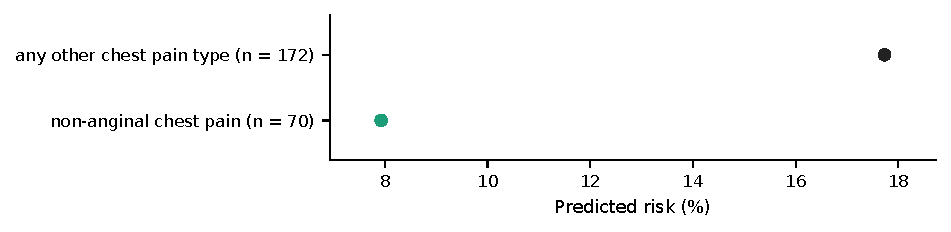
\includegraphics[width=\linewidth,height=0.88\textheight,keepaspectratio]{figures/heart-s1-c1/ann_30-categories-small.pdf}
\caption{Non-anginal chest pain relay: The predicted value for the typical case at each level, through this part (n = training patients; grey: fewer than 20).}
\label{fig:hearts1c1:plot-ann30-0}
\end{figure}
\begin{figure}[H]\centering
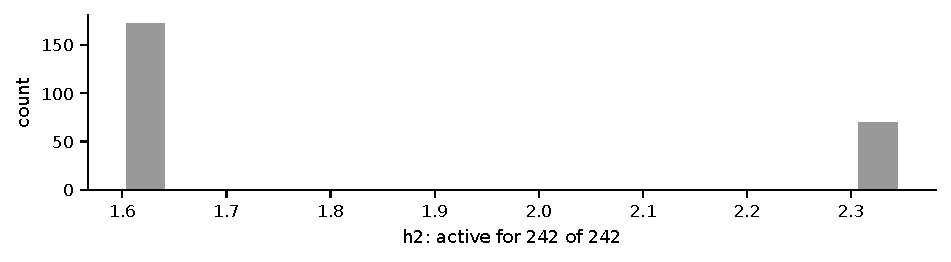
\includegraphics[width=\linewidth,height=0.88\textheight,keepaspectratio]{figures/heart-s1-c1/ann_30-units.pdf}
\caption{Non-anginal chest pain relay: This part's hidden units: each unit's output against its main numeric input (top) and how often it is active (bottom).}
\label{fig:hearts1c1:plot-ann30-1}
\end{figure}
\par\smallskip\noindent{\small Technical detail: \ref{tech:ann30}.\par}
\subsubsection{Maximum heart rate}\label{rd:ann32}
\noindent{\footnotesize Part of: The whole model (\ref{rd:ann34}).\par}
\noindent{\small Figure~\ref{fig:hearts1c1:parts-ann32} shows what feeds this part; Figure~\ref{fig:hearts1c1:units-ann32} its units and every connection into them (dashed boxes: connections from or to other parts, drawn in their own sections).\par}
\begin{figure}[H]\centering
\resizebox{!}{\ifdim\height>0.5\textheight 0.5\textheight\else\height\fi}{%
\resizebox{\ifdim\width>\linewidth\linewidth\else\width\fi}{!}{%
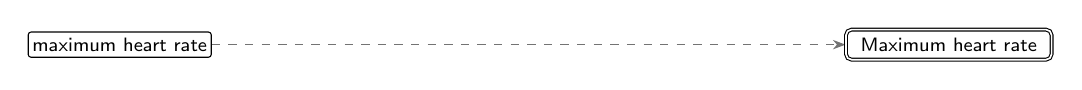
\begin{tikzpicture}[
  font=\sffamily\scriptsize, >={Stealth[length=1.6mm]},
  inp/.style={draw, rounded corners=1pt, fill=white, inner sep=1.5pt, minimum height=3.2mm, anchor=east},
  abox/.style={draw, thick, rounded corners=2pt, align=center, inner sep=3pt, minimum height=6mm, text width=42mm},
  outp/.style={draw, double, rounded corners=2pt, fill=white, align=center, inner sep=3pt, text width=24mm},
  agg/.style={draw=black!55},
]
\node[inp] (i0) at (0,-0.0) {maximum heart rate};
\node[outp] (out) at (9.36,0) {Maximum heart rate};
\begin{scope}[on background layer]
\draw[->, agg, thin, dashed] (i0.east) -- (out.west);
\end{scope}
\end{tikzpicture}}}%
\caption{Maximum heart rate: what feeds it, one level down.}
\label{fig:hearts1c1:parts-ann32}
\end{figure}
\begin{figure}[H]\centering
\resizebox{\ifdim\width>\linewidth\linewidth\else\width\fi}{!}{%
\definecolor{netup}{HTML}{D95F02}\definecolor{netdown}{HTML}{1B9E77}\definecolor{netmixed}{HTML}{7F7F7F}%
\begin{tikzpicture}[
  font=\sffamily\scriptsize, >={Stealth[length=1.4mm]},
  inp/.style={draw, circle, fill=white, minimum size=3.2mm, inner sep=0pt},
  hid/.style={draw, circle, fill=white, minimum size=5.2mm, inner sep=0.5pt, font=\sffamily\tiny},
  exitbox/.style={draw, thick, rectangle, fill=white, align=center, text width=17mm, minimum height=5mm, inner sep=1.5pt, font=\sffamily\tiny},
  sumbox/.style={draw, thick, dashed, rectangle, fill=white, align=center, text width=17mm, minimum height=5mm, inner sep=1.5pt, font=\sffamily\tiny},
  outp/.style={draw, thick, regular polygon, regular polygon sides=6, fill=white, minimum size=10mm, inner sep=0pt, font=\sffamily\tiny, align=center},
  stub/.style={draw, dashed, rounded corners=2pt, fill=white, align=center, inner sep=2pt, font=\sffamily\tiny, text width=15mm},
  inlab/.style={font=\sffamily\tiny, align=center, text width=15mm, inner sep=1pt, fill=white, fill opacity=0.8, text opacity=1},
  wpos/.style={draw=NavyBlue}, wneg/.style={draw=BrickRed}, wagg/.style={draw=black!45, line width=1.2pt},
  wmix/.style={draw=Plum},
]
\node[hid] (n2650) at (1.8,3.25) {h6};
\node[hid] (n2009) at (1.8,1.9) {h4};
\node[inp, draw=netdown, very thick] (ninxxthalach) at (1.8,0.0) {};
\path (ninxxthalach.south) node[inlab, anchor=north] (labninxxthalach) {max heart rate $\downarrow$};
\node[stub] (ntoxxthexmodelxoutput) at (1.8,4.8) {to the model output};
\begin{scope}[on background layer]
\node[fit=(n2650) (n2009) , inner sep=8pt, rounded corners=5pt, fill=Cerulean!10, draw=Cerulean!45] (clu0) {};
\draw[->, wpos, line width=0.59pt] (n2009) -- (n2650);
\draw[->, wpos, line width=0.54pt] (ninxxthalach) -- (n2009);
\draw[->, wneg, line width=0.30pt] (n2009) -- (ntoxxthexmodelxoutput);
\draw[->, wneg, line width=0.31pt] (n2650) -- (ntoxxthexmodelxoutput);
\end{scope}
\node[font=\sffamily\scriptsize\bfseries, text=Cerulean!55!black, anchor=south west, inner sep=1pt, fill=white, fill opacity=0.85, text opacity=1] at (clu0.north west) {Maximum heart rate};
\end{tikzpicture}}%
\caption{Maximum heart rate: its units and every connection into them. Blue: positive weight (raises the score); red: negative weight (lowers it); thicker: larger weight. Orange outline and up arrow: raises the final prediction; teal and down arrow: lowers it; grey and double arrow: depends.}
\label{fig:hearts1c1:units-ann32}
\end{figure}
\paragraph{Hypothesis.} This part lowers the predicted risk for a higher maximum heart rate: nothing until about 145 beats per minute, then steadily.\,{\scriptsize\textcolor{NavyBlue}{[C45, C46]}}
\paragraph{Evidence.} Through it, a higher maximum heart rate takes a typical patient from about 19\% at 71 to about 13\% at 182 beats per minute, with nothing until about 145 beats per minute, then steadily.\,{\scriptsize\textcolor{NavyBlue}{[C46]}} Its formula reproduces the part exactly on all 242 training patients.\,{\scriptsize\textcolor{NavyBlue}{[C47]}}
\par\noindent{\small Evidence plots: Figure~\ref{fig:hearts1c1:plot-ann32-0}, Figure~\ref{fig:hearts1c1:plot-ann32-1}, Figure~\ref{fig:hearts1c1:plot-ann32-2}, Figure~\ref{fig:hearts1c1:plot-ann32-3}.\par}
\par\noindent{\small Figure~\ref{fig:hearts1c1:plot-ann32-1} shows this part's own output, unit h4: it switches on at about 144.7 beats per minute of maximum heart rate, and is zero below.\par}
\par\noindent{\small Figure~\ref{fig:hearts1c1:plot-ann32-2} shows this part's own output, unit h6.\par}
\begin{figure}[H]\centering
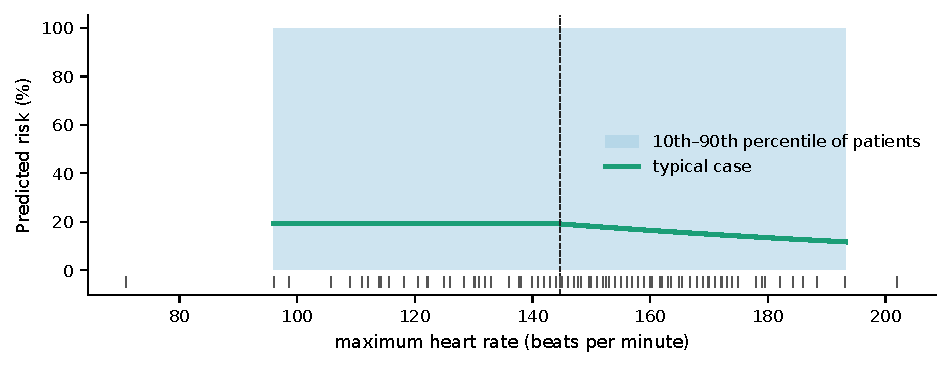
\includegraphics[width=\linewidth,height=0.88\textheight,keepaspectratio]{figures/heart-s1-c1/ann_32-response.pdf}
\caption{Maximum heart rate: Response curves through this part: the typical case (bold), the 10th to 90th percentile of individual patients (band), the fold or step point (dashed) with its spread across them (grey), and the observed values (ticks).}
\label{fig:hearts1c1:plot-ann32-0}
\end{figure}
\begin{figure}[H]\centering
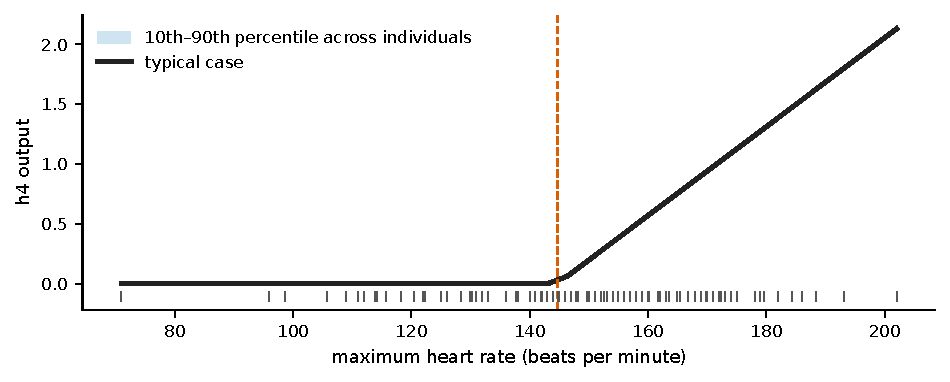
\includegraphics[width=\linewidth,height=0.88\textheight,keepaspectratio]{figures/heart-s1-c1/ann_32-partial-2009.pdf}
\caption{Maximum heart rate: This part's own output, unit h4 (the output of 'Maximum heart rate'), on its own scale (its activation), with every other input at the typical case; it is active for 155 of 242. Bold: the typical case; band: 10th to 90th percentile across individuals; dashed: where it switches on; ticks: the data.}
\label{fig:hearts1c1:plot-ann32-1}
\end{figure}
\begin{figure}[H]\centering
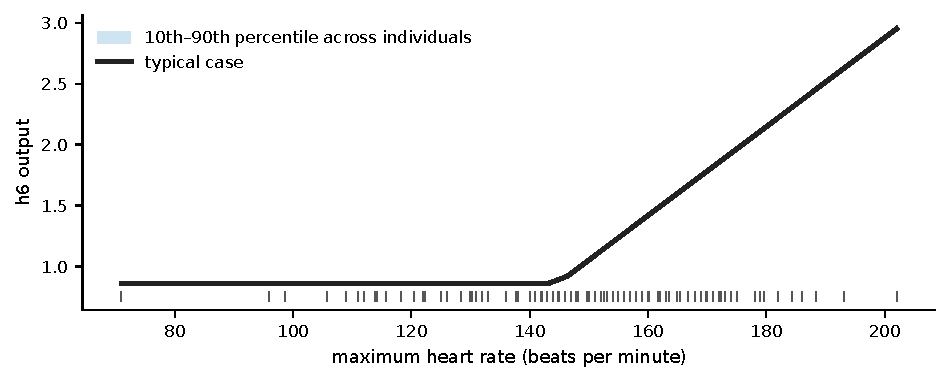
\includegraphics[width=\linewidth,height=0.88\textheight,keepaspectratio]{figures/heart-s1-c1/ann_32-partial-2650.pdf}
\caption{Maximum heart rate: This part's own output, unit h6 (the output of 'Maximum heart rate'), on its own scale (its activation), with every other input at the typical case; it is active for 242 of 242. Bold: the typical case; band: 10th to 90th percentile across individuals; ticks: the data.}
\label{fig:hearts1c1:plot-ann32-2}
\end{figure}
\begin{figure}[H]\centering
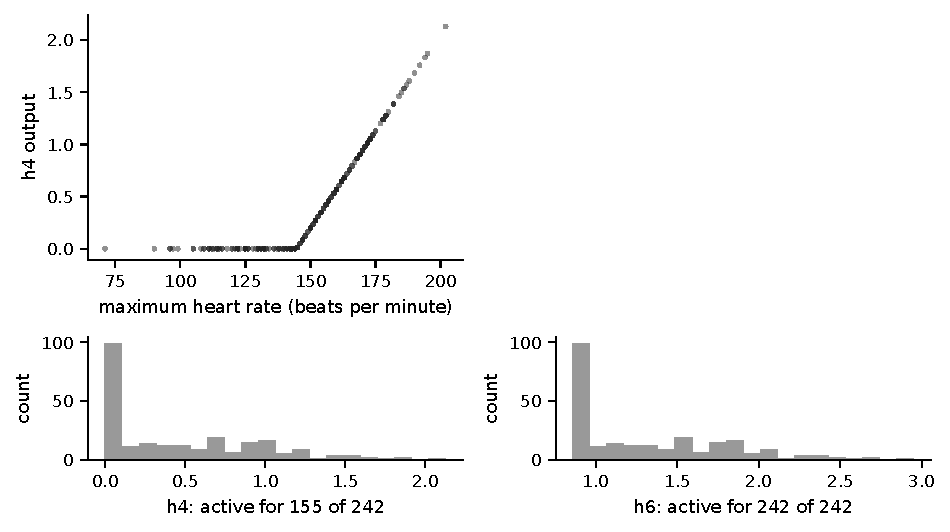
\includegraphics[width=\linewidth,height=0.88\textheight,keepaspectratio]{figures/heart-s1-c1/ann_32-units.pdf}
\caption{Maximum heart rate: This part's hidden units: each unit's output against its main numeric input (top) and how often it is active (bottom).}
\label{fig:hearts1c1:plot-ann32-3}
\end{figure}
\par\smallskip\noindent{\small Technical detail: \ref{tech:ann32}.\par}
\subsection{Not supported by the model}
\noindent{\small Every claim passed its checks.}
\clearpage\section*{Technical detail: heart-s1-c1}
\addcontentsline{toc}{section}{Technical detail: heart-s1-c1}
\noindent{\small The record behind each part: the original hypothesis, the closed form, and every claim with its estimate (log-odds and odds ratio), range across patients, n and test check.\par}
\renewcommand{\thesubsection}{T.\arabic{subsection}}\setcounter{subsection}{0}
\subsection{The whole model}\label{tech:ann34}
\noindent{\footnotesize Annotation ann\_\allowbreak{}34 (heart\_\allowbreak{}disease\_\allowbreak{}logit). Reads: age, sex, chest pain type, resting blood pressure, serum cholesterol, fasting blood sugar, resting ECG, maximum heart rate reached during the exercise test, exercise-induced angina, ST depression during exercise (compared with rest), slope of the ST segment at peak exercise, number of major vessels coloured by fluoroscopy, thallium stress test result.\par}
\paragraph{Original hypothesis (unchanged).} Hypothesis: the heart-disease logit is essentially a logistic regression. 13 direct input-$>$output edges (largest: sex:0 -1.87, slope:2 +1.72, ca +1.30, cp:4 +1.25, chol +0.93, thal:3 -0.87, thal:6 -0.86, trestbps +0.67, cp:2 +0.44, age +0.40, fbs:1 -0.32, slope:3 +0.20, thalach +0.002) are added to five children: ca\_\allowbreak{}slope2\_\allowbreak{}relay and the 2245 relay (raise the effective ca weight to 2.60 per SD), cp3\_\allowbreak{}relay (non-anginal pain lowers risk), st\_\allowbreak{}depression\_\allowbreak{}normal\_\allowbreak{}ecg\_\allowbreak{}gate (ST depression raises risk only with a normal resting ECG), typical\_\allowbreak{}angina\_\allowbreak{}ca\_\allowbreak{}switch's 3210 (typical angina lowers risk, less with more vessels) and max\_\allowbreak{}heart\_\allowbreak{}rate\_\allowbreak{}hinge (small). Nine inputs are unconnected (sex:1, fbs:0, restecg:1, restecg:2, exang:0, exang:1, slope:1, thal:4, thal:7): exercise-induced angina is ignored. Evidence (train, n=242): AUC 0.9392; all hidden units replaced by their best linear fits 0.9355 (= L2 logistic regression 0.9355); all ReLUs as identity 0.9078; all hidden mean-ablated 0.9241. The gain over linear (+0.0037) comes from the ECG/ST gate (+0.0034 restored alone), the heart-rate hinge (+0.0008) and the typical-angina switch (+0.0003); the relays contribute none. Direct edges carry logit SD 4.25 of 5.63.
\paragraph{Closed form.} Read through its parts (their formulas are in their own sections).
\paragraph{Split inputs.} To annotate the parts, the explanation split these inputs into copies (a refactoring step that does not change what the model computes); the diagrams draw each input once: vessels (3 copies); flat ST (2 copies); max heart rate (2 copies).
\paragraph{Evidence table} (next page, landscape).
\begin{landscape}
{\scriptsize\setlength{\tabcolsep}{3pt}\renewcommand{\arraystretch}{1.15}
\rowcolors{2}{black!6}{white}
\begin{longtable}{@{}l>{\raggedright\arraybackslash}p{0.36\linewidth}>{\raggedright\arraybackslash}p{0.14\linewidth}rrr>{\raggedright\arraybackslash}p{0.06\linewidth}>{\raggedright\arraybackslash}p{0.17\linewidth}c@{}}
\toprule\rowcolor{white}
ID & What is checked & Risk, typical patient & Log-odds & OR & Range (p10--p90) & n & Test check & OK \\
\midrule\endfirsthead
\toprule\rowcolor{white}
ID & What is checked & Risk, typical patient & Log-odds & OR & Range (p10--p90) & n & Test check & OK \\
\midrule\endhead
\bottomrule\endfoot
C01 & direction: number of vessels coloured by fluoroscopy: 0 vessels to 2 vessels (whole model) \newline{\itshape shape: steady (equal steps); 100\% of patients same; verified; risk saturates near 100\%} & 18\% to 99\% & 5.89 & 362 & 5.83 to 5.83 & 242 & unclear; AUC gain 0.041 [-0.032, 0.123] & \textcolor{OliveGreen}{yes} \\
C02 & direction: slope of the ST segment at peak exercise: an upsloping ST segment to a flat ST segment (whole model) \newline{\itshape shape: categorical; highest to lowest: a flat ST segment, a downsloping ST segment, an upsloping ST segment} & 18\% to 91\% & 3.81 & 44.9 & 3.81 to 3.81 & 115, 110 & disagrees; AUC gain -0.011 [-0.065, 0.036] & \textcolor{OliveGreen}{yes} \\
C03 & direction: slope of the ST segment at peak exercise: an upsloping ST segment to a flat ST segment (direct contribution only, not through any part) \newline{\itshape shape: categorical; highest to lowest: a flat ST segment, a downsloping ST segment, an upsloping ST segment} & 18\% to 87\% & 3.46 & 31.9 & 3.46 to 3.46 & 115, 110 & disagrees; AUC gain -0.012 [-0.059, 0.030] & \textcolor{OliveGreen}{yes} \\
C04 & direction: number of vessels coloured by fluoroscopy: 0 vessels to 2 vessels (direct contribution only, not through any part) \newline{\itshape shape: steady (equal steps); 100\% of patients same; verified} & 18\% to 80\% & 2.91 & 18.3 & 2.91 to 2.91 & 242 & disagrees; AUC gain -0.001 [-0.039, 0.032] & \textcolor{OliveGreen}{yes} \\
C05 & direction: thallium stress test result: a normal thallium scan to thallium stress test result other than a normal thallium scan, a fixed defect on the thallium scan (whole model) \newline{\itshape shape: categorical; highest to lowest: thallium stress test result other than a normal thallium scan, a fixed defect on the thallium scan, a normal thallium scan, a fixed defect on the thallium scan} & 18\% to 55\% & 1.74 & 5.71 & 1.74 to 1.74 & 135, 92 & unclear; AUC gain 0.012 [-0.017, 0.044] & \textcolor{OliveGreen}{yes} \\
C06 & direction: ST depression on exercise: 0.0 mm to 2.8 mm (whole model) \newline{\itshape shape: hinge at 1.0 mm; 100\% of patients same; fallback; matches the fold at 1.0 mm} & 18\% to 55\% & 0.87 & 2.38 & 0.00 to 1.74 & 242 & unclear; AUC gain 0.005 [-0.005, 0.022] & \textcolor{OliveGreen}{yes} \\
C07 & direction: serum cholesterol: 193 mg/dL (5.0 mmol/L) to 308 mg/dL (8.0 mmol/L) (whole model) \newline{\itshape shape: steady; 100\% of patients same; verified} & 8\% to 45\% & 2.22 & 9.23 & 2.22 to 2.22 & 242 & disagrees; AUC gain -0.022 [-0.066, 0.011] & \textcolor{OliveGreen}{yes} \\
C08 & direction: resting blood pressure: 110 mm Hg to 155 mm Hg (whole model) \newline{\itshape shape: steady; 100\% of patients same; verified} & 9\% to 35\% & 1.65 & 5.20 & 1.65 to 1.65 & 242 & unclear; AUC gain 0.000 [-0.022, 0.020] & \textcolor{OliveGreen}{yes} \\
C09 & direction: chest pain type: no chest pain (asymptomatic) to typical angina (whole model) \newline{\itshape shape: categorical; highest to lowest: no chest pain (asymptomatic), atypical angina, non-anginal chest pain, typical angina} & 18\% to $<$1\% & -4.55 & 0.01 & -4.78 to -4.08 & 108, 22 & agrees; AUC gain 0.041 [0.003, 0.083] & \textcolor{OliveGreen}{yes} \\
C10 & direction: sex: male to female (whole model) \newline{\itshape shape: categorical; highest to lowest: male, female} & 18\% to $<$1\% & -3.94 & 0.02 & -3.94 to -3.94 & 159, 83 & unclear; AUC gain 0.023 [-0.014, 0.068] & \textcolor{OliveGreen}{yes} \\
C11 & direction: chest pain type: no chest pain (asymptomatic) to non-anginal chest pain (whole model) \newline{\itshape shape: categorical; highest to lowest: no chest pain (asymptomatic), atypical angina, non-anginal chest pain, typical angina} & 18\% to 1\% & -3.43 & 0.03 & -3.43 to -3.43 & 108, 70 & agrees; AUC gain 0.041 [0.003, 0.083] & \textcolor{OliveGreen}{yes} \\
C12 & direction: chest pain type: no chest pain (asymptomatic) to chest pain type other than atypical angina, no chest pain (asymptomatic) (direct contribution only, not through any part) \newline{\itshape shape: categorical; highest to lowest: no chest pain (asymptomatic), atypical angina, chest pain type other than atypical angina, no chest pain (asymptomatic)} & 18\% to 2\% & -2.51 & 0.08 & -2.51 to -2.51 & 108, 92 & agrees; AUC gain 0.037 [0.006, 0.074] & \textcolor{OliveGreen}{yes} \\
C13 & direction: age: 42 years to 66 years (whole model) \newline{\itshape shape: steady; 100\% of patients same; verified} & 10\% to 25\% & 1.05 & 2.87 & 1.05 to 1.05 & 242 & disagrees; AUC gain -0.008 [-0.018, 0.001] & \textcolor{OliveGreen}{yes} \\
C14 & direction: thallium stress test result: a normal thallium scan to a fixed defect on the thallium scan (whole model) \newline{\itshape shape: categorical; highest to lowest: thallium stress test result other than a normal thallium scan, a fixed defect on the thallium scan, a normal thallium scan, a fixed defect on the thallium scan} & 18\% to 3\% & -1.83 & 0.16 & -1.83 to -1.83 & 135, 15 (small n) & unclear; AUC gain 0.012 [-0.017, 0.044] & \textcolor{OliveGreen}{yes} \\
C15 & direction: slope of the ST segment at peak exercise: an upsloping ST segment to a downsloping ST segment (direct contribution only, not through any part) \newline{\itshape shape: categorical; highest to lowest: a flat ST segment, a downsloping ST segment, an upsloping ST segment} & 18\% to 32\% & 0.77 & 2.16 & 0.77 to 0.77 & 115, 17 (small n) & disagrees; AUC gain -0.012 [-0.059, 0.030] & \textcolor{OliveGreen}{yes} \\
C16 & direction: slope of the ST segment at peak exercise: an upsloping ST segment to a downsloping ST segment (whole model) \newline{\itshape shape: categorical; highest to lowest: a flat ST segment, a downsloping ST segment, an upsloping ST segment} & 18\% to 32\% & 0.77 & 2.16 & 0.77 to 0.77 & 115, 17 (small n) & disagrees; AUC gain -0.011 [-0.065, 0.036] & \textcolor{OliveGreen}{yes} \\
C17 & direction: chest pain type: no chest pain (asymptomatic) to atypical angina (direct contribution only, not through any part) \newline{\itshape shape: categorical; highest to lowest: no chest pain (asymptomatic), atypical angina, chest pain type other than atypical angina, no chest pain (asymptomatic)} & 18\% to 5\% & -1.34 & 0.26 & -1.34 to -1.34 & 108, 42 & agrees; AUC gain 0.037 [0.006, 0.074] & \textcolor{OliveGreen}{yes} \\
C18 & direction: chest pain type: no chest pain (asymptomatic) to atypical angina (whole model) \newline{\itshape shape: categorical; highest to lowest: no chest pain (asymptomatic), atypical angina, non-anginal chest pain, typical angina} & 18\% to 5\% & -1.34 & 0.26 & -1.34 to -1.34 & 108, 42 & agrees; AUC gain 0.041 [0.003, 0.083] & \textcolor{OliveGreen}{yes} \\
C19 & direction: fasting blood sugar: fasting blood sugar of 120 mg/dL or less to fasting blood sugar above 120 mg/dL (whole model) \newline{\itshape shape: categorical; highest to lowest: fasting blood sugar of 120 mg/dL or less, fasting blood sugar above 120 mg/dL} & 18\% to 8\% & -0.92 & 0.40 & -0.92 to -0.92 & 209, 33 & disagrees; AUC gain -0.001 [-0.010, 0.009] & \textcolor{OliveGreen}{yes} \\
C20 & direction: maximum heart rate: 118 beats per minute to 175 beats per minute (whole model) \newline{\itshape shape: hinge at 145 beats per minute; 100\% of patients same; verified; matches the fold at 145 beats per minute} & 19\% to 14\% & -0.36 & 0.70 & -0.36 to -0.36 & 242 & unclear; AUC gain 0.002 [0.000, 0.009] & \textcolor{OliveGreen}{yes} \\
C21 & direction: maximum heart rate: 118 beats per minute to 175 beats per minute (direct contribution only, not through any part) \newline{\itshape shape: flat; 100\% of patients same; verified} & 18\% to 18\% & 0.005 & 1.00 & 0.005 to 0.005 & 242 & unclear; AUC gain 0.000 [0.000, 0.000] & \textcolor{OliveGreen}{yes} \\
C22 & direction: resting ECG: a normal resting ECG to resting ECG other than a normal resting ECG (whole model) \newline{\itshape shape: categorical; highest to lowest: a normal resting ECG, resting ECG other than a normal resting ECG} & 18\% to 18\% & -0.46 & 0.63 & -1.74 to 0.00 & 121, 121 & disagrees; AUC gain -0.008 [-0.021, 0.000] & \textcolor{OliveGreen}{yes} \\
C23 & magnitude: number of vessels coloured by fluoroscopy: 0 vessels to 2 vessels, typical patient \newline{\itshape shape: steady (equal steps); 100\% of patients same; verified; risk saturates near 100\%} & 18\% to 99\% & 5.83 & 340 &  & 242 & unclear; AUC gain 0.041 [-0.032, 0.123] & \textcolor{OliveGreen}{yes} \\
C24 & magnitude: slope of the ST segment at peak exercise: an upsloping ST segment to a flat ST segment, typical patient \newline{\itshape shape: categorical; highest to lowest: a flat ST segment, a downsloping ST segment, an upsloping ST segment} & 18\% to 91\% & 3.81 & 44.9 &  & 115, 110 & disagrees; AUC gain -0.011 [-0.065, 0.036] & \textcolor{OliveGreen}{yes} \\
C25 & magnitude: thallium stress test result: a normal thallium scan to thallium stress test result other than a normal thallium scan, a fixed defect on the thallium scan, typical patient \newline{\itshape shape: categorical; highest to lowest: thallium stress test result other than a normal thallium scan, a fixed defect on the thallium scan, a normal thallium scan, a fixed defect on the thallium scan} & 18\% to 55\% & 1.74 & 5.71 &  & 135, 92 & unclear; AUC gain 0.012 [-0.017, 0.044] & \textcolor{OliveGreen}{yes} \\
C26 & magnitude: ST depression on exercise: 0.0 mm to 2.8 mm, typical patient \newline{\itshape shape: hinge at 1.0 mm; 100\% of patients same; fallback; matches the fold at 1.0 mm} & 18\% to 55\% & 1.74 & 5.68 &  & 242 & unclear; AUC gain 0.005 [-0.005, 0.022] & \textcolor{OliveGreen}{yes} \\
C27 & magnitude: serum cholesterol: 193 mg/dL (5.0 mmol/L) to 308 mg/dL (8.0 mmol/L), typical patient \newline{\itshape shape: steady; 100\% of patients same; verified} & 8\% to 45\% & 2.22 & 9.23 &  & 242 & disagrees; AUC gain -0.022 [-0.066, 0.011] & \textcolor{OliveGreen}{yes} \\
C28 & null: model ignores exercise-induced angina (exact rule) &  & 0.00 &  &  & 242 & train only & \textcolor{OliveGreen}{yes} \\
C29 & structure: made of ca\_\allowbreak{}slope2\_\allowbreak{}relay, cp3\_\allowbreak{}relay, st\_\allowbreak{}depression\_\allowbreak{}normal\_\allowbreak{}ecg\_\allowbreak{}gate,\allowbreak{} max\_\allowbreak{}heart\_\allowbreak{}rate\_\allowbreak{}hinge,\allowbreak{} typical\_\allowbreak{}angina\_\allowbreak{}ca\_\allowbreak{}switch and inputs age, sex, cp, trestbps, chol, fbs, thalach, slope, ca, thal; added &  &  &  &  & 242 & train only & \textcolor{OliveGreen}{yes} \\
\end{longtable}}
\end{landscape}
\subsection{Typical angina with vessels}\label{tech:ann33}
\noindent{\footnotesize Annotation ann\_\allowbreak{}33 (typical\_\allowbreak{}angina\_\allowbreak{}ca\_\allowbreak{}switch). Reads: chest pain type, number of major vessels coloured by fluoroscopy.\par}
\paragraph{Original hypothesis (unchanged).} Hypothesis: (i) node 2245 = ReLU(0.578 ca + 1.276) is an always-on ca relay adding +0.88 logit per SD of ca (output weight 1.528); (ii) node 3210 = ReLU(0.901 cp:1 - 0.644*2245 + 0.420) is a typical-angina switch: it is on only for cp:1 patients and then lowers the logit by 0.833 x its activation, from about -2.26 at the lowest ca (-0.73 SD) to about -1.22 at the highest ca (2.64 SD). So typical angina lowers predicted risk, and the reduction shrinks with more narrowed vessels. Evidence (train, n=242): 2245 never clips (0.86..2.80); 3210 active for all 22 cp:1 patients and none of the 220 others. Mean ablation AUC 2245 0.9339, 3210 0.9354; linear replacement 0.9392 / 0.9391 (3210 is a cp:1 switch whose within-group response is linear in ca).
\paragraph{Closed form} {\footnotesize(weights and biases at 3 significant figures; largest difference from the part on the training patients 0.0).}
{\small\begingroup\allowdisplaybreaks
\begin{align*}
y_{0} &= \operatorname{relu}\bigl(1.28 + 0.578 x_{ca\_c}\bigr) \\
y_{1} &= \operatorname{relu}\bigl(0.42 + 0.901 x_{cp:1} - 0.644 \operatorname{relu}\bigl(1.28 \\
&\qquad + 0.578 x_{ca\_c}\bigr)\bigr)
\end{align*}\endgroup}

\paragraph{Evidence table} (next page, landscape).
\begin{landscape}
{\scriptsize\setlength{\tabcolsep}{3pt}\renewcommand{\arraystretch}{1.15}
\rowcolors{2}{black!6}{white}
\begin{longtable}{@{}l>{\raggedright\arraybackslash}p{0.36\linewidth}>{\raggedright\arraybackslash}p{0.14\linewidth}rrr>{\raggedright\arraybackslash}p{0.06\linewidth}>{\raggedright\arraybackslash}p{0.17\linewidth}c@{}}
\toprule\rowcolor{white}
ID & What is checked & Risk, typical patient & Log-odds & OR & Range (p10--p90) & n & Test check & OK \\
\midrule\endfirsthead
\toprule\rowcolor{white}
ID & What is checked & Risk, typical patient & Log-odds & OR & Range (p10--p90) & n & Test check & OK \\
\midrule\endhead
\bottomrule\endfoot
C30 & direction: number of vessels coloured by fluoroscopy: 0 vessels to 2 vessels (through this part) \newline{\itshape shape: steady (equal steps); 100\% of patients same; verified} & 18\% to 61\% & 2.04 & 7.73 & 1.98 to 1.98 & 242 & disagrees; AUC gain -0.003 [-0.032, 0.019] & \textcolor{OliveGreen}{yes} \\
C31 & direction: chest pain type: chest pain type other than typical angina to typical angina (through this part) \newline{\itshape shape: categorical; highest to lowest: chest pain type other than typical angina, typical angina} & 18\% to 2\% & -2.04 & 0.13 & -2.26 to -1.57 & 220, 22 & unclear; AUC gain 0.001 [-0.005, 0.008] & \textcolor{OliveGreen}{yes} \\
C32 & interaction: effect of number of vessels coloured by fluoroscopy (0 vessels to 2 vessels) by chest pain type: typical angina minus chest pain type other than typical angina; stronger in typical angina \newline{\itshape shape: steady (equal steps); 100\% of patients same; verified; risk saturates near 0\%} & typical angina: $<$1\% to 55\%; chest pain type other than typical angina: 18\% to 99\% & 0.70 & 2.00 &  & 22, 220 & agrees; AUC gain 0.001 [-0.005, 0.008] & \textcolor{OliveGreen}{yes} \\
C33 & structure: its formula reproduces it on 242 training patients (largest difference 0.0) &  & 0.00 &  &  & 242 & train only & \textcolor{OliveGreen}{yes} \\
\end{longtable}}
\end{landscape}
\subsection{ST depression with a normal ECG}\label{tech:ann31}
\noindent{\footnotesize Annotation ann\_\allowbreak{}31 (st\_\allowbreak{}depression\_\allowbreak{}normal\_\allowbreak{}ecg\_\allowbreak{}gate). Reads: resting ECG, ST depression during exercise (compared with rest).\par}
\paragraph{Original hypothesis (unchanged).} Hypothesis: node 1801 = ReLU(1.542 restecg:0 + 0.817 oldpeak - 1.521) is a gate in which ST depression (oldpeak) raises predicted risk only for patients with a normal resting ECG (restecg:0), once oldpeak is above about its mean (threshold -0.03 SD); with an abnormal resting ECG the threshold is 3.75 SD and the gate is effectively closed. Evidence (train, n=242): active for 41 of 121 normal-ECG patients and 1 of 121 others; adds 1.40 x activation = +1.14 logit per SD oldpeak when open. It is the model's main nonlinearity: mean ablation AUC 0.9339, linear replacement 0.9362, and restoring it onto the all-linear model gains +0.0034 AUC. oldpeak has no direct edge, so the model ignores ST depression for patients with an abnormal resting ECG.
\paragraph{Closed form} {\footnotesize(weights and biases at 3 significant figures; largest difference from the part on the training patients 2.22045e-16).}
{\small\begingroup\allowdisplaybreaks
\begin{align*}
y_{0} &= \operatorname{relu}\bigl(-1.52 + 1.54 x_{restecg:0} + 0.818 x_{oldpeak}\bigr)
\end{align*}\endgroup}

\paragraph{Evidence table} (next page, landscape).
\begin{landscape}
{\scriptsize\setlength{\tabcolsep}{3pt}\renewcommand{\arraystretch}{1.15}
\rowcolors{2}{black!6}{white}
\begin{longtable}{@{}l>{\raggedright\arraybackslash}p{0.36\linewidth}>{\raggedright\arraybackslash}p{0.14\linewidth}rrr>{\raggedright\arraybackslash}p{0.06\linewidth}>{\raggedright\arraybackslash}p{0.17\linewidth}c@{}}
\toprule\rowcolor{white}
ID & What is checked & Risk, typical patient & Log-odds & OR & Range (p10--p90) & n & Test check & OK \\
\midrule\endfirsthead
\toprule\rowcolor{white}
ID & What is checked & Risk, typical patient & Log-odds & OR & Range (p10--p90) & n & Test check & OK \\
\midrule\endhead
\bottomrule\endfoot
C34 & direction: ST depression on exercise: 0.0 mm to 2.8 mm (through this part) \newline{\itshape shape: hinge at 1.0 mm; 100\% of patients same; fallback; one point with C37 (median fold 1.0 mm, typical patient 1.0 mm, 10th-90th percentile 1.0 mm to 1.0 mm)} & 18\% to 55\% & 0.87 & 2.38 & 0.00 to 1.74 & 242 & unclear; AUC gain 0.005 [-0.005, 0.022] & \textcolor{OliveGreen}{yes} \\
C35 & direction: resting ECG: a normal resting ECG to resting ECG other than a normal resting ECG (through this part) \newline{\itshape shape: categorical; highest to lowest: a normal resting ECG, resting ECG other than a normal resting ECG} & 99\% to 98\% (typical patient this part acts on) & -0.46 & 0.63 & -1.74 to 0.00 & 121, 121 & disagrees; AUC gain -0.008 [-0.021, 0.000] & \textcolor{OliveGreen}{yes} \\
C36 & interaction: effect of ST depression on exercise (0.0 mm to 2.8 mm) by resting ECG: resting ECG other than a normal resting ECG minus a normal resting ECG; stronger in a normal resting ECG \newline{\itshape shape: hinge at 1.0 mm; 100\% of patients same; fallback} & resting ECG other than a normal resting ECG: 18\% to 18\%; a normal resting ECG: 18\% to 55\% & -1.74 & 0.18 &  & 121, 121 & agrees; AUC gain -0.008 [-0.021, 0.000] & \textcolor{OliveGreen}{yes} \\
C37 & threshold: ST depression on exercise: fold at about 1.0 mm (starts) for patients with a normal resting ECG \newline{\itshape shape: hinge at 1.0 mm; 100\% of patients same; fallback; one point with C37 (median fold 1.0 mm, typical patient 1.0 mm, 10th-90th percentile 1.0 mm to 1.0 mm)} & 13\% to 63\% (typical patient with a fold (patients with a normal resting ECG)) & 2.41 & 11.1 & 2.41 to 2.41 & 121, 41 & unclear; AUC gain 0.005 [-0.005, 0.022] & \textcolor{OliveGreen}{yes} \\
C38 & subgroup: who this part acts on: 42 of 242 patients & 98\% to 99\% (typical patient this part acts on (risk without the part, then with it)) & 1.08 & 2.95 & 0.19 to 2.50 & 42, 200 & unclear; AUC gain 0.005 [-0.006, 0.025] & \textcolor{OliveGreen}{yes} \\
C39 & structure: its formula reproduces it on 242 training patients (largest difference 2.22045e-16) &  & 2e-16 &  &  & 242 & train only & \textcolor{OliveGreen}{yes} \\
\end{longtable}}
\end{landscape}
\subsection{Vessels with flat ST segment}\label{tech:ann29}
\noindent{\footnotesize Annotation ann\_\allowbreak{}29 (ca\_\allowbreak{}slope2\_\allowbreak{}relay). Reads: slope of the ST segment at peak exercise, number of major vessels coloured by fluoroscopy.\par}
\paragraph{Original hypothesis (unchanged).} Hypothesis: node 664 = ReLU(0.456 ca + 0.185 slope:2 + 0.783) is an affine relay that strengthens the direct ca and flat-ST-slope (slope:2) effects. Evidence (train, n=242): pre-activation 0.28..2.19, never clips, so the part is exactly affine on the data; it adds +0.42 logit per SD of ca and +0.17 per SD of slope:2 (output weight 0.92). Mean ablation AUC 0.9392 -$>$ 0.9375; linear replacement leaves AUC at 0.9392. No concept beyond reweighting.
\paragraph{Closed form} {\footnotesize(weights and biases at 3 significant figures; largest difference from the part on the training patients 2.22045e-16).}
{\small\begingroup\allowdisplaybreaks
\begin{align*}
y_{0} &= \operatorname{relu}\bigl(0.783 + 0.185 x_{slope:2\_b} + 0.456 x_{ca\_b}\bigr)
\end{align*}\endgroup}

\paragraph{Evidence table} (next page, landscape).
\begin{landscape}
{\scriptsize\setlength{\tabcolsep}{3pt}\renewcommand{\arraystretch}{1.15}
\rowcolors{2}{black!6}{white}
\begin{longtable}{@{}l>{\raggedright\arraybackslash}p{0.36\linewidth}>{\raggedright\arraybackslash}p{0.14\linewidth}rrr>{\raggedright\arraybackslash}p{0.06\linewidth}>{\raggedright\arraybackslash}p{0.17\linewidth}c@{}}
\toprule\rowcolor{white}
ID & What is checked & Risk, typical patient & Log-odds & OR & Range (p10--p90) & n & Test check & OK \\
\midrule\endfirsthead
\toprule\rowcolor{white}
ID & What is checked & Risk, typical patient & Log-odds & OR & Range (p10--p90) & n & Test check & OK \\
\midrule\endhead
\bottomrule\endfoot
C40 & direction: number of vessels coloured by fluoroscopy: 0 vessels to 2 vessels (through this part) \newline{\itshape shape: steady (equal steps); 100\% of patients same; verified} & 18\% to 36\% & 0.94 & 2.56 & 0.94 to 0.94 & 242 & disagrees; AUC gain -0.002 [-0.019, 0.011] & \textcolor{OliveGreen}{yes} \\
C41 & direction: slope of the ST segment at peak exercise: slope of the ST segment at peak exercise other than a flat ST segment to a flat ST segment (through this part) \newline{\itshape shape: categorical; highest to lowest: a flat ST segment, slope of the ST segment at peak exercise other than a flat ST segment} & 18\% to 23\% & 0.34 & 1.41 & 0.34 to 0.34 & 132, 110 & disagrees; AUC gain -0.003 [-0.016, 0.005] & \textcolor{OliveGreen}{yes} \\
C42 & structure: its formula reproduces it on 242 training patients (largest difference 2.22045e-16) &  & 2e-16 &  &  & 242 & train only & \textcolor{OliveGreen}{yes} \\
\end{longtable}}
\end{landscape}
\subsection{Non-anginal chest pain relay}\label{tech:ann30}
\noindent{\footnotesize Annotation ann\_\allowbreak{}30 (cp3\_\allowbreak{}relay). Reads: chest pain type.\par}
\paragraph{Original hypothesis (unchanged).} Hypothesis: node 1173 = ReLU(0.336 cp:3 + 1.818) is an always-on relay through which non-anginal chest pain (cp:3) lowers predicted risk. Evidence (train, n=242): pre-activation 1.60..2.34, never clips (entry-exit correlation 1.0); with output weight -1.24 it contributes -0.417 logit per SD of cp:3, about -0.92 logit for non-anginal pain vs other types. cp:3 has no direct edge, so this is its only route. Mean ablation AUC 0.9373; linear replacement 0.9392.
\paragraph{Closed form} {\footnotesize(weights and biases at 3 significant figures; largest difference from the part on the training patients 0.0).}
{\small\begingroup\allowdisplaybreaks
\begin{align*}
y_{0} &= \operatorname{relu}\bigl(1.82 + 0.336 x_{cp:3}\bigr)
\end{align*}\endgroup}

\paragraph{Evidence table} (next page, landscape).
\begin{landscape}
{\scriptsize\setlength{\tabcolsep}{3pt}\renewcommand{\arraystretch}{1.15}
\rowcolors{2}{black!6}{white}
\begin{longtable}{@{}l>{\raggedright\arraybackslash}p{0.36\linewidth}>{\raggedright\arraybackslash}p{0.14\linewidth}rrr>{\raggedright\arraybackslash}p{0.06\linewidth}>{\raggedright\arraybackslash}p{0.17\linewidth}c@{}}
\toprule\rowcolor{white}
ID & What is checked & Risk, typical patient & Log-odds & OR & Range (p10--p90) & n & Test check & OK \\
\midrule\endfirsthead
\toprule\rowcolor{white}
ID & What is checked & Risk, typical patient & Log-odds & OR & Range (p10--p90) & n & Test check & OK \\
\midrule\endhead
\bottomrule\endfoot
C43 & direction: chest pain type: chest pain type other than non-anginal chest pain to non-anginal chest pain (through this part) \newline{\itshape shape: categorical; highest to lowest: chest pain type other than non-anginal chest pain, non-anginal chest pain} & 18\% to 8\% & -0.92 & 0.40 & -0.92 to -0.92 & 172, 70 & unclear; AUC gain 0.001 [-0.008, 0.013] & \textcolor{OliveGreen}{yes} \\
C44 & structure: its formula reproduces it on 242 training patients (largest difference 0.0) &  & 0.00 &  &  & 242 & train only & \textcolor{OliveGreen}{yes} \\
\end{longtable}}
\end{landscape}
\subsection{Maximum heart rate}\label{tech:ann32}
\noindent{\footnotesize Annotation ann\_\allowbreak{}32 (max\_\allowbreak{}heart\_\allowbreak{}rate\_\allowbreak{}hinge). Reads: maximum heart rate reached during the exercise test.\par}
\paragraph{Original hypothesis (unchanged).} Hypothesis: a small hinge on maximum heart rate (thalach). Node 2009 = ReLU(0.833 thalach + 0.201) feeds the output (-0.151) and the always-on relay 2650 = ReLU(0.982*2009 + 0.859) (-0.172), a net -0.32 x 2009: higher maximum heart rate lowers predicted risk, but only above about -0.24 SD; below that it has no effect (the direct thalach edge, +0.002, is negligible). Evidence (train, n=242): 2009 active for 64\% of patients; logit contribution SD 0.16 (small); mean ablation AUC 0.9391, linear replacement 0.9392, restore-onto-linear gain +0.0008.
\paragraph{Closed form} {\footnotesize(weights and biases at 3 significant figures; largest difference from the part on the training patients 0.0).}
{\small\begingroup\allowdisplaybreaks
\begin{align*}
y_{0} &= \operatorname{relu}\bigl(0.201 + 0.833 x_{thalach\_b}\bigr) \\
y_{1} &= \operatorname{relu}\bigl(0.859 + 0.982 \operatorname{relu}\bigl(0.201 \\
&\qquad + 0.833 x_{thalach\_b}\bigr)\bigr)
\end{align*}\endgroup}

\paragraph{Evidence table} (next page, landscape).
\begin{landscape}
{\scriptsize\setlength{\tabcolsep}{3pt}\renewcommand{\arraystretch}{1.15}
\rowcolors{2}{black!6}{white}
\begin{longtable}{@{}l>{\raggedright\arraybackslash}p{0.36\linewidth}>{\raggedright\arraybackslash}p{0.14\linewidth}rrr>{\raggedright\arraybackslash}p{0.06\linewidth}>{\raggedright\arraybackslash}p{0.17\linewidth}c@{}}
\toprule\rowcolor{white}
ID & What is checked & Risk, typical patient & Log-odds & OR & Range (p10--p90) & n & Test check & OK \\
\midrule\endfirsthead
\toprule\rowcolor{white}
ID & What is checked & Risk, typical patient & Log-odds & OR & Range (p10--p90) & n & Test check & OK \\
\midrule\endhead
\bottomrule\endfoot
C45 & direction: maximum heart rate: 118 beats per minute to 175 beats per minute (through this part) \newline{\itshape shape: hinge at 145 beats per minute; 100\% of patients same; verified; one point with C46 (median fold 145 beats per minute, typical patient 145 beats per minute, 10th-90th percentile 145 beats per minute to 145 beats per minute)} & 19\% to 14\% & -0.36 & 0.70 & -0.36 to -0.36 & 242 & unclear; AUC gain 0.002 [0.000, 0.009] & \textcolor{OliveGreen}{yes} \\
C46 & threshold: maximum heart rate: fold at about 145 beats per minute (starts) \newline{\itshape shape: hinge at 145 beats per minute; 100\% of patients same; verified; one point with C46 (median fold 145 beats per minute, typical patient 145 beats per minute, 10th-90th percentile 145 beats per minute to 145 beats per minute)} & 19\% to 13\% (typical patient with a fold) & -0.44 & 0.64 & -0.44 to -0.44 & 242, 155 & unclear; AUC gain 0.002 [0.000, 0.009] & \textcolor{OliveGreen}{yes} \\
C47 & structure: its formula reproduces it on 242 training patients (largest difference 0.0) &  & 0.00 &  &  & 242 & train only & \textcolor{OliveGreen}{yes} \\
\end{longtable}}
\end{landscape}
\subsection*{The network before any explanation}\addcontentsline{toc}{subsection}{The network before any explanation} Figure~\ref{fig:hearts1c1:raw} (next page, landscape) is the trained network as it is, with no parts, no splits and no inserted units: inputs at the bottom, hidden units by depth, the output at the top, every connection drawn, every input column its own node (one-hot levels included).
\begin{landscape}
\begin{figure}[p]\centering
\resizebox{\linewidth}{!}{%
\definecolor{netup}{HTML}{D95F02}\definecolor{netdown}{HTML}{1B9E77}\definecolor{netmixed}{HTML}{7F7F7F}%
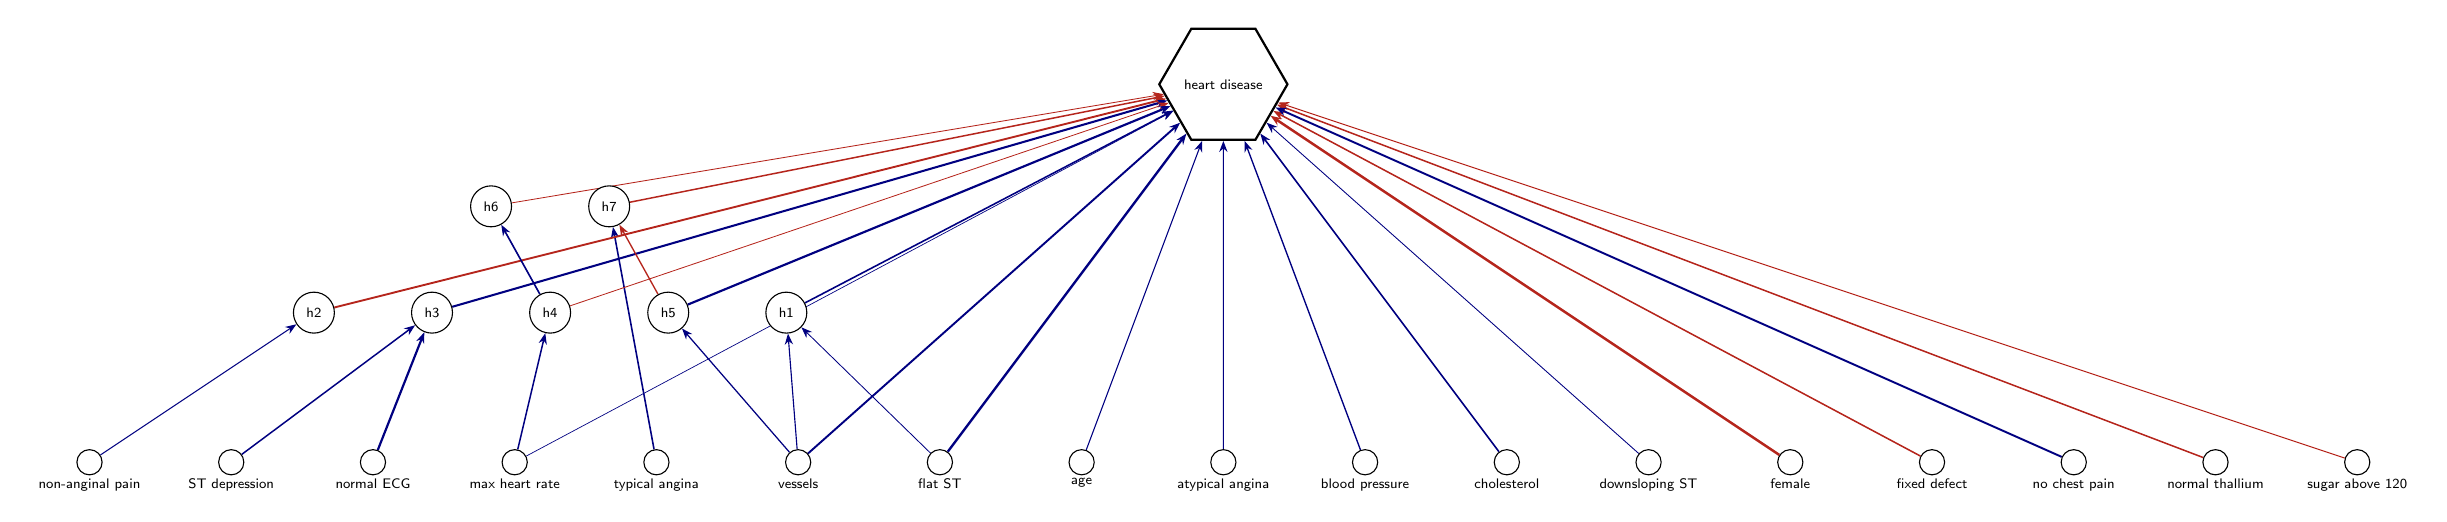
\begin{tikzpicture}[
  font=\sffamily\scriptsize, >={Stealth[length=1.4mm]},
  inp/.style={draw, circle, fill=white, minimum size=3.2mm, inner sep=0pt},
  hid/.style={draw, circle, fill=white, minimum size=5.2mm, inner sep=0.5pt, font=\sffamily\tiny},
  exitbox/.style={draw, thick, rectangle, fill=white, align=center, text width=17mm, minimum height=5mm, inner sep=1.5pt, font=\sffamily\tiny},
  sumbox/.style={draw, thick, dashed, rectangle, fill=white, align=center, text width=17mm, minimum height=5mm, inner sep=1.5pt, font=\sffamily\tiny},
  outp/.style={draw, thick, regular polygon, regular polygon sides=6, fill=white, minimum size=10mm, inner sep=0pt, font=\sffamily\tiny, align=center},
  stub/.style={draw, dashed, rounded corners=2pt, fill=white, align=center, inner sep=2pt, font=\sffamily\tiny, text width=15mm},
  inlab/.style={font=\sffamily\tiny, align=center, text width=15mm, inner sep=1pt, fill=white, fill opacity=0.8, text opacity=1},
  wpos/.style={draw=NavyBlue}, wneg/.style={draw=BrickRed}, wagg/.style={draw=black!45, line width=1.2pt},
  wmix/.style={draw=Plum},
]
\node[inp] (ninxxage) at (12.6,0.0) {};
\path (ninxxage.south) node[inlab, anchor=north] (labninxxage) {age};
\node[inp] (ninxxfbsx1) at (28.8,0.0) {};
\path (ninxxfbsx1.south) node[inlab, anchor=north] (labninxxfbsx1) {sugar above 120};
\node[inp] (ninxxrestecgx0) at (3.6,0.0) {};
\path (ninxxrestecgx0.south) node[inlab, anchor=north] (labninxxrestecgx0) {normal ECG};
\node[inp] (ninxxthalach) at (5.4,0.0) {};
\path (ninxxthalach.south) node[inlab, anchor=north] (labninxxthalach) {max heart rate};
\node[inp] (ninxxoldpeak) at (1.8,0.0) {};
\path (ninxxoldpeak.south) node[inlab, anchor=north] (labninxxoldpeak) {ST depression};
\node[inp] (ninxxsexx0) at (21.6,0.0) {};
\path (ninxxsexx0.south) node[inlab, anchor=north] (labninxxsexx0) {female};
\node[inp] (ninxxslopex2) at (10.8,0.0) {};
\path (ninxxslopex2.south) node[inlab, anchor=north] (labninxxslopex2) {flat ST};
\node[inp] (ninxxslopex3) at (19.8,0.0) {};
\path (ninxxslopex3.south) node[inlab, anchor=north] (labninxxslopex3) {downsloping ST};
\node[inp] (ninxxca) at (9.0,0.0) {};
\path (ninxxca.south) node[inlab, anchor=north] (labninxxca) {vessels};
\node[inp] (ninxxthalx3) at (27.0,0.0) {};
\path (ninxxthalx3.south) node[inlab, anchor=north] (labninxxthalx3) {normal thallium};
\node[inp] (ninxxthalx6) at (23.4,0.0) {};
\path (ninxxthalx6.south) node[inlab, anchor=north] (labninxxthalx6) {fixed defect};
\node[inp] (ninxxcpx1) at (7.2,0.0) {};
\path (ninxxcpx1.south) node[inlab, anchor=north] (labninxxcpx1) {typical angina};
\node[inp] (ninxxcpx2) at (14.4,0.0) {};
\path (ninxxcpx2.south) node[inlab, anchor=north] (labninxxcpx2) {atypical angina};
\node[inp] (ninxxcpx3) at (0.0,0.0) {};
\path (ninxxcpx3.south) node[inlab, anchor=north] (labninxxcpx3) {non-anginal pain};
\node[inp] (ninxxcpx4) at (25.2,0.0) {};
\path (ninxxcpx4.south) node[inlab, anchor=north] (labninxxcpx4) {no chest pain};
\node[inp] (ninxxtrestbps) at (16.2,0.0) {};
\path (ninxxtrestbps.south) node[inlab, anchor=north] (labninxxtrestbps) {blood pressure};
\node[inp] (ninxxchol) at (18.0,0.0) {};
\path (ninxxchol.south) node[inlab, anchor=north] (labninxxchol) {cholesterol};
\node[outp] (n0) at (14.4,4.8) {heart disease};
\node[hid] (n1173) at (2.85,1.9) {h2};
\node[hid] (n1801) at (4.35,1.9) {h3};
\node[hid] (n2009) at (5.85,1.9) {h4};
\node[hid] (n2245) at (7.35,1.9) {h5};
\node[hid] (n2650) at (5.1,3.25) {h6};
\node[hid] (n3210) at (6.6,3.25) {h7};
\node[hid] (n664) at (8.85,1.9) {h1};
\begin{scope}[on background layer]
\draw[->, wpos, line width=0.39pt] (ninxxage) -- (n0);
\draw[->, wneg, line width=0.36pt] (ninxxfbsx1) -- (n0);
\draw[->, wpos, line width=0.79pt] (ninxxrestecgx0) -- (n1801);
\draw[->, wpos, line width=0.25pt] (ninxxthalach) -- (n0);
\draw[->, wpos, line width=0.54pt] (ninxxthalach) -- (n2009);
\draw[->, wpos, line width=0.54pt] (ninxxoldpeak) -- (n1801);
\draw[->, wneg, line width=0.90pt] (ninxxsexx0) -- (n0);
\draw[->, wpos, line width=0.85pt] (ninxxslopex2) -- (n0);
\draw[->, wpos, line width=0.31pt] (ninxxslopex2) -- (n664);
\draw[->, wpos, line width=0.32pt] (ninxxslopex3) -- (n0);
\draw[->, wpos, line width=0.70pt] (ninxxca) -- (n0);
\draw[->, wpos, line width=0.45pt] (ninxxca) -- (n2245);
\draw[->, wpos, line width=0.41pt] (ninxxca) -- (n664);
\draw[->, wneg, line width=0.55pt] (ninxxthalx3) -- (n0);
\draw[->, wneg, line width=0.55pt] (ninxxthalx6) -- (n0);
\draw[->, wpos, line width=0.57pt] (ninxxcpx1) -- (n3210);
\draw[->, wpos, line width=0.41pt] (ninxxcpx2) -- (n0);
\draw[->, wpos, line width=0.37pt] (ninxxcpx3) -- (n1173);
\draw[->, wpos, line width=0.69pt] (ninxxcpx4) -- (n0);
\draw[->, wpos, line width=0.48pt] (ninxxtrestbps) -- (n0);
\draw[->, wpos, line width=0.58pt] (ninxxchol) -- (n0);
\draw[->, wneg, line width=0.68pt] (n1173) -- (n0);
\draw[->, wpos, line width=0.74pt] (n1801) -- (n0);
\draw[->, wneg, line width=0.30pt] (n2009) -- (n0);
\draw[->, wpos, line width=0.59pt] (n2009) -- (n2650);
\draw[->, wpos, line width=0.78pt] (n2245) -- (n0);
\draw[->, wneg, line width=0.48pt] (n2245) -- (n3210);
\draw[->, wneg, line width=0.31pt] (n2650) -- (n0);
\draw[->, wneg, line width=0.54pt] (n3210) -- (n0);
\draw[->, wpos, line width=0.57pt] (n664) -- (n0);
\end{scope}
\end{tikzpicture}}%
\caption{The network as trained, before any explanation, in full. Blue: positive weight (raises the score); red: negative weight (lowers it); thicker: larger weight. Orange outline and up arrow: raises the final prediction; teal and down arrow: lowers it; grey and double arrow: depends. Not used (no connection): male, sugar 120 or less, ST-T abnormal ECG, LVH on ECG, no exercise pain, exercise pain, upsloping ST, thallium code 4, reversible defect.}
\label{fig:hearts1c1:raw}
\end{figure}
\end{landscape}
\end{drafted}
\clearpage
\end{document}
